\documentclass{article}
% ========================================================================
% ===== 中文相关 =====
\usepackage[UTF8,noindent]{ctex}     %  引入 ctex 宏包，支持中文排版
\usepackage{xeCJKfntef,xcolor}       %  引入 xeCJKfntef 宏包用于处理 CJK 字体，xcolor 用于颜色支持
\xeCJKsetup{underdot/symbol=^^b7}    %  设置下划点符号为中点（·）
\newfontfamily\kaisu{STKaiti}        %  定义新字体命令 \kaisu，使用 STKaiti 字体（楷书）
\setCJKsansfont{simkai.ttf}          %  设置 CJK 无衬线字体为 simkai.ttf（仿宋）
\setCJKmonofont{STKaiti}             %  设置 CJK 等宽字体为 STKaiti（楷书）
% ===== 西文字体 =====
\setsansfont{TeX Gyre Termes}        %  设置无衬线字体为 TeX Gyre Termes
\setmonofont{TeX Gyre Termes}        %  设置等宽字体为 TeX Gyre Termes
% ========================================================================
\usepackage{amssymb}
\usepackage{graphics}
\usepackage{graphicx}
%%%%%% H-N %%%%%%
\usepackage{mathdots}
\usepackage{mathtools}
\usepackage{mathrsfs}
\usepackage{multicol}
%%%%%% O-T %%%%%%
\usepackage{pstricks}
\usepackage{tikz}
\usepackage{tkz-euclide}
%%%%%% U-Z %%%%%%
\usepackage[all,poly,knot]{xy}
\usepackage{ifthen}
% ========================================================================
\usetikzlibrary{math,shapes.geometric,quotes,angles,calc,decorations.pathreplacing}
% ========================================================================
\newcommand{\nc}{\newcommand}
\newcommand{\on}[1]{\operatorname{#1}}
% ========================================================================
% ========== list of symbols ===========
\nc{\fraka}{{\mathfrak a}}
\nc{\frakb}{{\mathfrak b}}
\nc{\frakc}{{\mathfrak c}}
\nc{\frakd}{{\mathfrak d}}
\nc{\frake}{{\mathfrak e}}
\nc{\frakf}{{\mathfrak f}}
\nc{\frakg}{{\mathfrak g}}
\nc{\frakh}{{\mathfrak h}}
\nc{\fraki}{{\mathfrak i}}
\nc{\frakj}{{\mathfrak j}}
\nc{\frakk}{{\mathfrak k}}
\nc{\frakl}{{\mathfrak l}}
\nc{\frakm}{{\mathfrak m}}
\nc{\frakn}{{\mathfrak n}}
\nc{\frako}{{\mathfrak o}}
\nc{\frakp}{{\mathfrak p}}
\nc{\frakq}{{\mathfrak q}}
\nc{\frakr}{{\mathfrak r}}
\nc{\fraks}{{\mathfrak s}}
\nc{\frakt}{{\mathfrak t}}
\nc{\fraku}{{\mathfrak u}}
\nc{\frakv}{{\mathfrak v}}
\nc{\frakw}{{\mathfrak w}}
\nc{\frakx}{{\mathfrak x}}
\nc{\fraky}{{\mathfrak y}}
\nc{\frakz}{{\mathfrak z}}
\nc{\frakA}{{\mathfrak A}}
\nc{\frakB}{{\mathfrak B}}
\nc{\frakC}{{\mathfrak C}}
\nc{\frakD}{{\mathfrak D}}
\nc{\frakE}{{\mathfrak E}}
\nc{\frakF}{{\mathfrak F}}
\nc{\frakG}{{\mathfrak G}}
\nc{\frakH}{{\mathfrak H}}
\nc{\frakI}{{\mathfrak I}}
\nc{\frakJ}{{\mathfrak J}}
\nc{\frakK}{{\mathfrak K}}
\nc{\frakL}{{\mathfrak L}}
\nc{\frakM}{{\mathfrak V}}
\nc{\frakN}{{\mathfrak N}}
\nc{\frakO}{{\mathfrak O}}
\nc{\frakP}{{\mathfrak P}}
\nc{\frakQ}{{\mathfrak Q}}
\nc{\frakR}{{\mathfrak R}}
\nc{\frakS}{{\mathfrak S}}
\nc{\frakT}{{\mathfrak T}}
\nc{\frakU}{{\mathfrak U}}
\nc{\frakV}{{\mathfrak V}}
\nc{\frakW}{{\mathfrak W}}
\nc{\frakX}{{\mathfrak X}}
\nc{\frakY}{{\mathfrak Y}}
\nc{\frakZ}{{\mathfrak Z}}
\nc{\bA}{{\mathbb A}}
\nc{\bB}{{\mathbb B}}
\nc{\bC}{{\mathbb C}}
\nc{\bD}{{\mathbb D}}
\nc{\bE}{{\mathbb E}}
\nc{\bF}{{\mathbb F}}
\nc{\bG}{{\mathbb G}}
\nc{\bH}{{\mathbb H}}
\nc{\bI}{{\mathbb I}}
\nc{\bJ}{{\mathbb J}}
\nc{\bK}{{\mathbb K}}
\nc{\bL}{{\mathbb L}}
\nc{\bM}{{\mathbb M}}
\nc{\bN}{{\mathbb N}}
\nc{\bO}{{\mathbb O}}
\nc{\bP}{{\mathbb P}}
\nc{\bQ}{{\mathbb Q}}
\nc{\bR}{{\mathbb R}}
\nc{\bS}{{\mathbb S}}
\nc{\bT}{{\mathbb T}}
\nc{\bU}{{\mathbb U}}
\nc{\bV}{{\mathbb V}}
\nc{\bW}{{\mathbb W}}
\nc{\bX}{{\mathbb X}}
\nc{\bY}{{\mathbb Y}}
\nc{\bZ}{{\mathbb Z}}
\nc{\mA}{{\mathcal A}}
\nc{\mB}{{\mathcal B}}
\nc{\mC}{{\mathcal C}}
\nc{\mD}{{\mathcal D}}
\nc{\mE}{{\mathcal E}}
\nc{\mF}{{\mathcal F}}
\nc{\mG}{{\mathcal G}}
\nc{\mH}{{\mathcal H}}
\nc{\mI}{{\mathcal I}}
\nc{\mJ}{{\mathcal J}}
\nc{\mK}{{\mathcal K}}
\nc{\mL}{{\mathcal L}}
\nc{\mM}{{\mathcal V}}
\nc{\mN}{{\mathcal N}}
\nc{\mO}{{\mathcal O}}
\nc{\mP}{{\mathcal P}}
\nc{\mQ}{{\mathcal Q}}
\nc{\mR}{{\mathcal R}}
\nc{\mS}{{\mathcal S}}
\nc{\mT}{{\mathcal T}}
\nc{\mU}{{\mathcal U}}
\nc{\mV}{{\mathcal V}}
\nc{\mW}{{\mathcal W}}
\nc{\mX}{{\mathcal X}}
\nc{\mY}{{\mathcal Y}}
\nc{\mZ}{{\mathcal Z}}
\nc{\sA}{{\mathscr A}}
\nc{\sB}{{\mathscr B}}
\nc{\sC}{{\mathscr C}}
\nc{\sD}{{\mathscr D}}
\nc{\sE}{{\mathscr E}}
\nc{\sF}{{\mathscr F}}
\nc{\sG}{{\mathscr G}}
\nc{\sH}{{\mathscr H}}
\nc{\sI}{{\mathscr I}}
\nc{\sJ}{{\mathscr J}}
\nc{\sK}{{\mathscr K}}
\nc{\sL}{{\mathscr L}}
\nc{\sM}{{\mathscr V}}
\nc{\sN}{{\mathscr N}}
\nc{\sO}{{\mathscr O}}
\nc{\sP}{{\mathscr P}}
\nc{\sQ}{{\mathscr Q}}
\nc{\sR}{{\mathscr R}}
\nc{\sS}{{\mathscr S}}
\nc{\sT}{{\mathscr T}}
\nc{\sU}{{\mathscr U}}
\nc{\sV}{{\mathscr V}}
\nc{\sW}{{\mathscr W}}
\nc{\sX}{{\mathscr X}}
\nc{\sY}{{\mathscr Y}}
\nc{\sZ}{{\mathscr Z}}
%%%%%%%%%%%%%%%%%%%%%%%%%%%%%%%%%%%%%%%%%%%%%%%%%%%%%%%%%%%%%%%%%%%%%%%%
% ===== 数学运算符 =====
\DeclareMathOperator{\Aut}{Aut}
\DeclareMathOperator{\rmd}{d}
\DeclareMathOperator{\End}{End}
\DeclareMathOperator{\Hom}{Hom}
\DeclareMathOperator{\Frac}{Frac}
\DeclareMathOperator{\Fil}{Fil}
\DeclareMathOperator{\Gal}{Gal}
\DeclareMathOperator{\GL}{GL}
\DeclareMathOperator{\Gr}{Gr}
\DeclareMathOperator{\PGL}{PGL}
\DeclareMathOperator{\Spec}{Spec}
\DeclareMathOperator{\rank}{rank}
% =============================
\nc{\cech} {{\check{\mathrm{C}}\mathrm{ech}}}
\nc{\mEnd} {{\on{\mathcal{E}\mathrm{nd}}}}
\nc{\gl}   {{\on{\mathfrak  {gl}}}}
\nc{\mHom} {{\on{\mathcal{H}\mathrm{om}}}}
\nc{\id}   {{\on{\mathrm  {id}}}}
%%%%%%%%%%%%%%%%%%%%%%%%%%%%%%%%%%%%%%%%%%%%%%%%%%%%%%%%%%%%%%%%%%%%%%%%
\newtheorem{theorem}{定理}  % 先定义 theorem 环境
\newtheorem{proposition}[theorem]{性质}  % 共享 theorem 的计数器
\newtheorem{question}[theorem]{问题}
\newtheorem{definition}[theorem]{定义}
\newtheorem{corollary}[theorem]{推论}
\newtheorem{lemma}[theorem]{引理}
%%%%%%%%%%%%%%%%%%%%%%%%%%%%%%%%%%%%%%%%%%%%%%%%%%%%%%%%%%%%%%%%%%%%%%%%
% ===== 颜色系统 =====
\renewcommand{\blue }[1]{{\textcolor[rgb]{0,0,1}{#1}}}
%\def\red{ }
%%%%%%%%%%%%%%%%%%%%%%%%%%%%%%%%%%%%%%%%%%%%%%%%%%%%%%%%%%%%%%%%%%%%%%%%
\begin{document}
\title{线性代数 \quad 中国科学技术大学}

\maketitle



\section{向量}


\subsection{向量及其运算}

\subsubsection{什么是向量}
\blue{向量} = 既有\underline{大小},又有\underline{方向}的量.

\subsubsection{向量加法}
\begin{definition}[向量的加法---平行四边形法则或者三角形法则]
\begin{equation*}
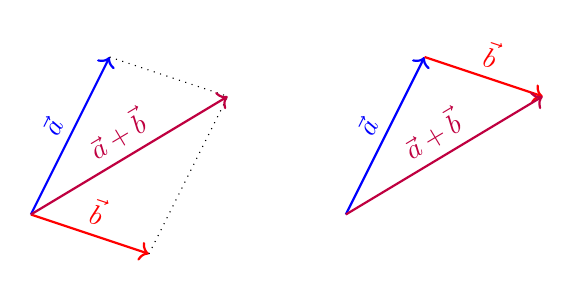
\begin{tikzpicture}[scale=1]
\tikzmath{\r=4;};
\coordinate (O) at (0,0);
\coordinate (A) at (1,2);
\coordinate (B) at (1.5,-0.5);
\coordinate (C) at (2.5,1.5);
\coordinate (o) at (0+\r,0);
\coordinate (a) at (1+\r,2);
\coordinate (b) at (1.5+\r,-0.5);
\coordinate (c) at (2.5+\r,1.5);
\draw[->,thick,blue](O)--(A) node[pos=.5,sloped,above] {$\vec{a}$};
\draw[->,thick,red](O)--(B) node[pos=.5,sloped,above] {$\vec{b}$};
\draw[dotted](A)--(C);
\draw[dotted](B)--(C);
\draw[->,thick,purple](O)--(C) node[pos=.5,sloped,above] {$\vec{a}+\vec{b}$};
\draw[->,thick,blue](o)--(a) node[pos=.5,sloped,above] {$\vec{a}$};
\draw[->,thick,red](a)--(c) node[pos=.5,sloped,above] {$\vec{b}$};
\draw[->,thick,purple](o)--(c) node[pos=.5,sloped,above] {$\vec{a}+\vec{b}$};
\end{tikzpicture}
\end{equation*}
\end{definition}

\subsubsection{向量减法}
\begin{definition}[向量的减法]
\[\vec{a}-\vec{b}:=\vec{a}+(-\vec{b}).\]
\end{definition}
\begin{equation*}
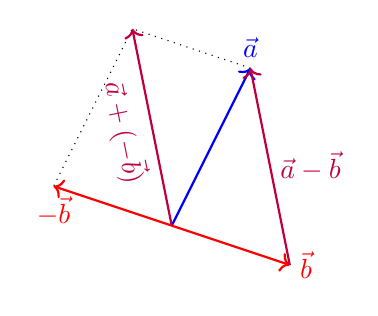
\begin{tikzpicture}[scale=1]
\coordinate (O) at (0,0);
\coordinate (A) at (1,2);
\coordinate (B) at (1.5,-0.5);
\coordinate (b) at (-1.5,0.5);
\coordinate (C) at (-0.5,2.5);
\draw[->,thick,blue](O)--(A) node[pos=1,above] {$\vec{a}$};
\draw[->,thick,red](O)--(B) node[pos=1,right] {$\vec{b}$};
\draw[->,thick,red](O)--(b) node[pos=1,below] {$-\vec{b}$};
\draw[dotted](A)--(C)--(b);
\draw[->,thick,purple](O)--(C) node[pos=0.5,sloped,below] {$\vec{a}+(-\vec{b})$};
\draw[->,thick,purple](B)--(A) node[pos=0.5,right] {$\vec{a}-\vec{b}$};
\end{tikzpicture}
\end{equation*}

\subsubsection{向量的数乘}
\begin{definition}[向量的数乘] 令$\vec{a}$为一向量, $\lambda$为一实数.\\
$\bullet$ 若$\lambda\geq0$,则$\lambda \vec{a}$定义为长度为$\lambda |\vec{a}|$且方向与$\vec{a}$相同的向量.\\
$\bullet$ 若$\lambda<0$,则$\lambda \vec{a}$定义为长度为$-\lambda |\vec{a}|$且方向与$\vec{a}$相反的向量.
\end{definition}
\begin{equation*}
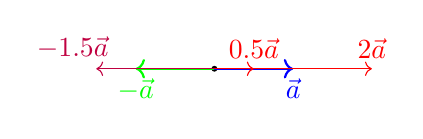
\begin{tikzpicture}[scale=1]
\coordinate (O) at (0,0);\draw [fill] (O) circle [radius=0.03];
\coordinate (A) at (1,0);
\coordinate (05A) at (0.5*1,0);
\coordinate (2A) at (2*1,0);
\coordinate (mA) at (-1*1,0);
\coordinate (m15A) at (-1.5*1,0);
\coordinate (B) at (-1,1);
\coordinate (mpiB) at (3.14,-3.14);
\coordinate (eB) at (-2.718,2.718);
\draw[->,thick,blue](O)--(A) node[pos=1,sloped,below] {$\vec{a}$};
\draw[->,red](O)--(05A) node[pos=1,sloped,above] {$0.5\vec{a}$};
\draw[->,red](O)--(2A) node[pos=1,sloped,above] {$2\vec{a}$};
\draw[->,thick,green](O)--(mA) node[pos=1,sloped,below] {$-\vec{a}$};
\draw[->,purple](O)--(m15A) node[pos=1.2,sloped,above] {$-1.5\vec{a}$};
\end{tikzpicture}
\end{equation*}

\subsubsection{线性运算}
\begin{definition}[线性运算]
向量的\blue{加法}和\blue{数乘}运算统称为向量的\blue{线性运算}.
\end{definition}
\begin{proposition}[向量线性运算的八条基本性质]
\begin{enumerate}
\item 加法交换律: $\vec{a}+\vec{b}=\vec{b}+\vec{a}$;
\item 加法结合律: $\vec{a}+(\vec{b}+\vec{c})=(\vec{a}+\vec{b})+\vec{c}$;
\item 存在零元: $\vec{a}+\vec{0}=\vec{a}=\vec{0}+\vec{a}$;
\item 存在负元: $\vec{a}+(-\vec{a})=\vec{0}=(-\vec{a})+\vec{a}$;
\item 数乘单位元: $1\vec{a} = \vec{a}$;
\item 数乘结合律: $\lambda(\mu \vec{a})=(\lambda \mu)\vec{a}$;
\item 左分配律: $(\lambda+\mu)\vec{a}=\lambda \vec{a} + \mu \vec{a}$;
\item 右分配律: $\lambda (\vec{a}+\vec{b}) =\lambda \vec{a} + \lambda \vec{b}$;
\end{enumerate}
\end{proposition}


\subsection{向量线性相关性}

\subsubsection{线性组合}
\begin{definition}[线性组合]
设 $\vec{a}_1$, $\vec{a}_2$, $\cdots$, $\vec{a}_m$  为一组向量, $\lambda_1$, $\lambda_2$, $\cdots$, $\lambda_m$ 为一组实数. 称向量
\[\lambda_1\vec{a}_1 + \lambda_2\vec{a}_2 + \cdots \lambda_m\vec{a}_m\]
为向量 $\vec{a}_1$, $\vec{a}_2$, $\cdots$, $\vec{a}_m$ 的\blue{线性组合}.
\end{definition}
也就是说,一组向量的线性组合就是从这组向量出发通过线性运算能够获得的向量.

\subsubsection{线性组合的几何解释}
\begin{center}\blue{\framebox(300,50){
$\xymatrix@R=0mm@C=3cm{
\text{空间} \ar@{<->}[r]_-{\text{固定一个点$O$(原点)}}^-{1:1}& \text{全体向量集}\\
P \ar@{|->}[r] & \overset{\longrightarrow}{OP}\\
}$}}
\end{center}
\begin{enumerate}
\item 设 $\vec{a}$为一个非零向量。则
\begin{center}
过原点与 $\vec{a}$ 平行的直线 \quad $\xleftrightarrow{\quad 1:1 \quad}$ \quad $\vec{a}$的全体线性组合.
\end{center}
\item 设$\vec{a},\vec{b}$不平行(不共线). 则
\begin{center}
过原点与 $\vec{a}$ 和 $\vec{b}$ 平行的平面 \quad $\xleftrightarrow{\quad 1:1 \quad}$\quad  $\vec{a},\vec{b}$ 的全体线性组合.
\end{center}
\end{enumerate}

\subsubsection{线性相关与线性无关}
\begin{definition}[线性相关,线性无关] 给定一组向量 $\vec{a}_1$, $\vec{a}_2$, $\cdots$, $\vec{a}_m$.
\begin{itemize}
\item 如果存在一组不全为零的实数 $\lambda_1$, $\lambda_2$, $\cdots$, $\lambda_m$ 使得
\[\lambda_1\vec{a}_1 + \lambda_2\vec{a}_2 + \cdots \lambda_m\vec{a}_m=\vec{0},\]
则称向量组$\vec{a}_1$, $\vec{a}_2$, $\cdots$, $\vec{a}_m$\blue{线性相关}.
\item 反之,若对任意一组不全为零的实数$\lambda_1$, $\lambda_2$, $\cdots$, $\lambda_m$都有
\[\lambda_1\vec{a}_1 + \lambda_2\vec{a}_2 + \cdots \lambda_m\vec{a}_m\neq \vec{0},\]
则称向量组 $\vec{a}_1$, $\vec{a}_2$, $\cdots$, $\vec{a}_m$的\blue{线性无关}.
\end{itemize}
\end{definition}

\subsubsection{线性相关的几何解释}
\begin{enumerate}
\item 一个向量$\vec{a}$线性相关 $\iff$ $\vec{a}=\vec0$;
\item 两个向量$\vec{a},\vec{b}$线性相关 $\iff$ $\vec{a}$与$\vec{b}$平行(共线);
\item 三个向量$\vec{a},\vec{b},\vec{c}$线性相关 $\iff$ $\vec{a},\vec{b},\vec{c}$共面;
\item 四个及四个以上的向量一定线性相关.
\end{enumerate}


\subsection{坐标系、坐标与坐标变换}

\subsubsection{仿射坐标系}
\begin{theorem}[向量的基本定理]
设$\vec{e}_1$, $\vec{e}_2$, $\vec{e}_3$ 为空间中的三个不共面的向量, 则对每个向量$\vec{a}$都\blue{存在唯一}的三元有序实数组$(x_1,x_2,x_3)$, 使得
\[\vec{a} = x_1\vec{e}_1 + x_2\vec{e}_2 + x_3\vec{e}_3.\]
\end{theorem}
\begin{definition}[基、坐标]
称不共面的三个向量$\vec{e}_1,\vec{e}_2,\vec{e}_3$为一组\blue{基}. 若
\[\vec{a} = x_1\vec{e}_1 + x_2\vec{e}_2 + x_3\vec{e}_3,\]
则称$(x_1,x_2,x_3)$为向量$\vec{a}$在基$\vec{e}_1,\vec{e}_2,\vec{e}_3$下的\blue{(仿射)坐标}.
\end{definition}
\begin{equation*}
\boxed{\blue{\text{仿射坐标系}}=\text{点} O  + \text{基} \vec{e}_1,\vec{e}_2,\vec{e}_3 \qquad \text{记作} \blue{[O;\vec{e}_1,\vec{e}_2,\vec{e}_3]}.}
\end{equation*}
\begin{corollary}[一一对应]
若给定仿射坐标系 $[O;\vec{e}_1,\vec{e}_2,\vec{e}_3]$,则有如下一一对应
\begin{center}\blue{\framebox(300,50){
$\xymatrix@R=0mm{
\text{空间} \ar@{<->}[r]^-{1:1}& \text{全体向量集} \ar@{<->}[r]^-{1:1} & \mathbb R^3=\mathbb R\times \mathbb R \times \mathbb R \\
P \ar@{|->}[r] & \overset{\longrightarrow}{OP} \ar@{|->}[r] & \text{坐标}(x_1,x_2,x_3) \\
}$}}
\end{center}
\end{corollary}

\subsubsection{向量的坐标运算}
给定仿射坐标系 $[O;\vec{e}_1,\vec{e}_2,\vec{e}_3]$, 我们用$(x_1,x_2,x_3)$表示向量$x_1\vec{e}_1+x_2\vec{e}_2+x_3\vec{e}_3$.
则我们有
\begin{proposition}
$\bullet$ $(x_1,x_2,x_3) + (y_1,y_2,y_3) = (x_1+y_1,x_2+y_2,x_3+y_3)$;\\
$\bullet$ $\lambda(x_1,x_2,x_3) = (\lambda x_1,\lambda x_2,\lambda x_3)$.
\end{proposition}

\subsubsection{坐标变换}
给定两个仿射坐标系 $[O;\vec{e}_1,\vec{e}_2,\vec{e}_3]$ 和 $[O';\vec{e}'_1,\vec{e}'_2,\vec{e}'_3]$.
设空间中的点$P$在两个坐标系下的坐标分别为 $(x,y,z)$ 和 $(x',y',z')$. 两个坐标之间的关系式
\begin{equation*}
\blue{\boxed{
\begin{split}
x' &= a_{11}x+a_{12}y+a_{13}z+x_0'\\
y' &= a_{21}x+a_{22}y+a_{23}z+y_0'\\
z' &= a_{31}x+a_{32}y+a_{33}z+z_0'\\
\end{split}
}}
\end{equation*}


\subsection{复数与数域}

\subsubsection{复数}
$\boxed{\xymatrix@R=4mm{
&\fbox{\text{\tiny 复数的代数表示}} &\sqrt{-1} \ar@<-1mm>[d]\\
z \ar@{}[r]|{=} & \underline{x} \ar@{}[r]|+ & \underline{i\ y}\\
&{\text{实部} \atop \mathrm{Re}z}\ar[u]&{\text{虚部}\atop \mathrm{Im}z}\ar[u]\\}}$

\boxed{\begin{tikzpicture}
\filldraw[black] (0,0) circle (2pt) node[below left]{$O$};
\filldraw[black] (2,1) circle (1pt) node[below]{};
\filldraw[black] (2,0) circle (1pt) node[below]{};
\filldraw[black] (0,1) circle (1pt) node[below]{};
\draw[black, thick,->]  (0,-0.5) -- (0,3) node[black,right]{虚轴};
\draw[black, thick,->]  (-0.5,0) -- (4,0) node[black,right]{实轴};
\draw[black, thick,dotted]  (2,1) -- (2,0) node[black,below]{$x$};
\draw[black, thick,dotted]  (2,1) -- (0,1) node[black,left]{$y$};
\draw[black, thick,->]  (0,0) -- (2,1) node[black,right]{${P(x,y) \atop z=x+iy}$};
\node[black] at (3.5,2.5){复平面};
\node[black] at (2,3.2){\fbox{\tiny 复数的几何表示}};
\node[black] at (0.8,0.2){$\theta$};
\node[black] at (1,0.7){$r$};
\draw[black, thick,-]  (0.44,0) -- (0.4,0.2);
\end{tikzpicture}}

\subsubsection{数域}
\begin{definition} 复数域的任意子集称为\blue{数集}. 若数集$\mathbb F$至少包含两个元素,且关于数的{\bf 加减乘除封闭},那么称$\mathbb F$为\blue{数域}.
\end{definition}
有理数集$\mathbb Q$,实数集$\mathbb R$,和复数集$\mathbb C$均为数域.


\subsection{数组向量}

\subsubsection{高维数组向量的定义}
设$\mathbb F$为数域, $n$为正整数.
\begin{definition}我们称一个由$n$个$\mathbb F$上的数$a_1,a_2,\cdots,a_n$组成的有序数组
\[\vec{a} := (a_1,\cdots,a_n)\]
为\blue{数域$\mathbb F$上的一个$n$维数组向量}.其中$a_i$称为$\vec{a}$的\blue{第$i$个分量}. 数域$\mathbb F$上$n$维数组向量全体记为 \blue{$\mathbb F^n$}.
\end{definition}


\subsubsection{高维数组向量的线性运算}
设 $\vec{a}=(a_1,\cdots,a_n)\in \mathbb F^n$, $\vec{b}=(b_1,\cdots,b_n)\in \mathbb F^n$, $\lambda\in \mathbb F$.
\begin{enumerate}
\item 加法: $\vec{a}+\vec{b}:=(a_1+b_1,a_2+b_2,\cdots,a_n+b_n)$.
\item 数乘: $\lambda \vec{a}:=(\lambda a_1,\lambda a_2,\cdots,\lambda a_n)$.
\item 零向量: $\vec{0}:=(0,\cdots,0)$.
\item 负向量: $-\vec{a}:=(-a_1,\cdots,-a_n)$.
\item 相等: $\vec{a}=\vec{b} \iff a_i=b_i \quad i=1,\cdots,n$.
\end{enumerate}
\blue{八条基本性质:}
\begin{enumerate}
\item 加法交换律: $\vec{a}+\vec{b}=\vec{b}+\vec{a}$;
\item 加法结合律: $\vec{a}+(\vec{b}+\vec{c})=(\vec{a}+\vec{b})+\vec{c}$;
\item 存在零元: $\vec{a}+\vec{0}=\vec{a}=\vec{0}+\vec{a}$;
\item 存在负元: $\vec{a}+(-\vec{a})=\vec{0}=(-\vec{a})+\vec{a}$;
\item 数乘单位元: $1\vec{a} = \vec{a}$;
\item 数乘结合律: $\lambda(\mu \vec{a})=(\lambda \mu)\vec{a}$;
\item 左分配律: $(\lambda+\mu)\vec{a}=\lambda \vec{a} + \mu \vec{a}$;
\item 右分配律: $\lambda (\vec{a}+\vec{b}) =\lambda \vec{a} + \lambda \vec{b}$;
\end{enumerate}

\subsubsection{线性相关(高维数组向量)}
设$\vec{a}_1,\vec{a}_2,\cdots,\vec{a}_n\in \mathbb F^n$,  $\lambda_1,\lambda_2,\cdots,\lambda_m\in \mathbb F$.
\begin{center}
\fbox{\blue{$\lambda_1\vec{a}_1 + \lambda_2\vec{a}_2 + \cdots \lambda_m\vec{a}_m$} \qquad $\longleftarrow$ \blue{线性组合} }
\end{center}
\begin{definition}[线性相关,线性无关]
一组向量 $\vec{a}_1$, $\vec{a}_2$, $\cdots$, $\vec{a}_m$ 称为\blue{线性相关}, 若存在一组不全为零的实数 $\lambda_1$, $\lambda_2$, $\cdots$, $\lambda_m$ 使得
\[\lambda_1\vec{a}_1 + \lambda_2\vec{a}_2 + \cdots \lambda_m\vec{a}_m=0.\]
反之,	则称向量 $\vec{a}_1$, $\vec{a}_2$, $\cdots$, $\vec{a}_m$的\blue{线性无关}.
\end{definition}

\newpage




\section{矩阵(一)}


\subsection{矩阵及其线性运算}

\subsubsection{矩阵的定义}
\begin{definition}[矩阵] 一个\blue{$m\times n$矩阵}为由 $m\times n$个数排成的$m$行$n$列的阵列
\[\left(
\begin{array}{cccc}
a_{11} & a_{12} & \cdots & a_{1 n}\\
a_{21} & a_{22} & \cdots & a_{2 n}\\
\vdots & \vdots & \ddots & \vdots\\
a_{m 1} & a_{m 2} & \cdots & a_{mn}\\
\end{array}
\right)_.\]
记作$A=(a_{ij})_{m\times n}$.  称 $a_{ij}$为矩阵$A$的\blue{第$(i,j)$元素};  当$i=j$时,$a_{ii}$也称为$A$的\blue{对角元}.
\end{definition}

\subsubsection{特殊矩阵命名}
按照矩阵行列数大小,非零元分布或元素取值范围等,我们有如下特殊矩阵命名:
\begin{enumerate}
\item $n$维\blue{行向量} := $1\times n$ 矩阵;
\item $n$维\blue{列向量} := $n\times 1$ 矩阵;
\item \blue{零矩阵} $O$, 或 $0$;
\item $n$阶\blue{方阵};
\item \blue{单位阵} $I$;
\item \blue{数量矩阵} $aI$;
\item \blue{对角矩阵} $\mathrm{diag}(a_1,\cdots,a_n)$;
\item \blue{上(下)三角矩阵};
\item \blue{(反)对称矩阵};
\item \blue{整数矩阵};\blue{有理数矩阵};\blue{实矩阵};\blue{复矩阵};
\item \blue{数域$\bF$上的矩阵};
\item \blue{多项式矩阵}.
\end{enumerate}

\subsubsection{矩阵的线性运算}
\begin{definition}[加法与数乘] 设$\lambda$为数域$\bF$中的数. 取两个$\bF$系数的$m\times n$矩阵 $A=(a_{ij})_{m\times n}\in \bF^{m\times n}$, $B=(b_{ij})_{m\times n}\in \bF^{m\times n}$.   定义
\begin{itemize}
\item \blue{加法}
\[\blue{A + B} :=(a_{ij}+b_{ij})_{m\times n}:=\begin{pmatrix}
a_{11}+b_{11} & a_{12}+b_{12} & \cdots & a_{1 n}+b_{1n}\\
a_{21}+b_{21} & a_{22}+b_{22} & \cdots & a_{2 n}+b_{2n}\\
\vdots & \vdots & \ddots & \vdots\\
a_{m 1}+b_{m1} & a_{m 2}+b_{m2} & \cdots & a_{mn}+b_{mn}
\end{pmatrix}_,\]
\item \blue{数乘}
\[\blue{\lambda A} :=(\lambda a_{ij})_{m\times n}:=\begin{pmatrix}
\lambda a_{11} & \lambda a_{12} & \cdots & \lambda a_{1 n}\\
\lambda a_{21} & \lambda a_{22} & \cdots & \lambda a_{2 n}\\
\vdots & \vdots & \ddots & \vdots\\
\lambda a_{m 1} & \lambda a_{m 2} & \cdots & \lambda a_{mn}
\end{pmatrix}_.\]
\end{itemize}
类似地定义\blue{负矩阵}和矩阵的\blue{减法}运算:
\[\blue{-A}:=(-a_{ij})_{m\times n}, \quad \blue{A-B}:=A+(-B) = (a_{ij}-b_{ij})_{m\times n}.\]
\end{definition}

\subsubsection{矩阵的线性运算}
类似于向量的线性运算,矩阵的线性运算也满足如下八条基本性质:
\begin{theorem}
\begin{enumerate}
\item 加法交换律: $A+B=B+A$;
\item 加法结合律: $A+(B+C)=(A+B)+C$;
\item 有零矩阵: $A+0=A=0+A$;
\item 有负矩阵: $A+(-A)=0=(-A)+A$;
\item 数乘单位元: $1A = A$;
\item 数乘结合律: $\lambda(\mu A)=(\lambda \mu)A$;
\item 左分配律: $(\lambda+\mu)A=\lambda A + \mu A$;
\item 右分配律: $\lambda (A+B) =\lambda A + \lambda B$;
\end{enumerate}
其中 $A,B,C$ 为使得运算有有意义的矩阵, $\lambda,\mu$为数.
\end{theorem}

\subsubsection{基本矩阵}
\begin{equation*}
\begin{array}{lcc}
E_{ij}:=& \left(\begin{array}{ccc}0&\cdots&0\\\vdots&1&\vdots\\0&\cdots&0\\\end{array}\right)
& \leftarrow\text{\small 第$i$行} \\
&{\uparrow \atop \text{第$j$列}} & \\
\end{array}
\end{equation*}
\begin{lemma}
任意 $m\times n$矩阵$A=(a_{ij})_{m\times n}$都可以唯一的表示为基本矩阵的线性组合
\[A=\sum_{i=1}^m\sum_{j=1}^n a_{ij}E_{ij}.\]
\end{lemma}


\subsection{矩阵乘法}

\subsubsection{数组向量空间之间的线性映射}
\begin{definition}[线性映射]
给定一个数组向量空间之间的映射$\sA\colon \bF^n\rightarrow \bF^m$.  若$\sA$满足
\begin{equation}\label{equ:linearoperator}\tag{$*$}
\begin{split}
\blue{\text{(保持加法)\quad }} &\sA(\vec{a} + \vec{b}) = \sA(\vec{a}) + \sA(\vec{b});\\
\blue{\text{(保持数乘)\quad }} &\sA(\lambda\vec{a}) = \lambda\sA(\vec{a})
\end{split}
\end{equation}
则$\sA$称为\blue{线性映射}.
\end{definition}

\subsubsection{矩阵与线性映射}
\begin{center}
\fbox{
$\bF^{m\times n}$ $\quad$ $\xleftrightarrow{\quad 1:1\quad }$ \quad
从$\bF^n$到$\bF^m$的全体线性映射.}
\end{center}
\begin{lemma}
线性映射的合成仍然是线性映射.
\end{lemma}

\subsubsection{矩阵的乘法}
\begin{definition}[矩阵乘法]设 $A=(a_{ik})_{m\times n}\in \bF^{m\times n}$,$B=(b_{kj})_{n\times p}\in \bF^{n\times p}$. 定义
\[\blue{AB}:=\left(\sum_{k=1}^{n}a_{ik}b_{kj}\right)_{m\times p}\in \bF^{m\times p}.\]
\end{definition}
注: 设$A$和$B$为线性映射$\mathscr A$和$\mathscr B$对应的矩阵. 则$\mathscr A\circ\mathscr B$ 对应的矩阵为 $AB$.

\subsubsection{矩阵乘法运算的基本性质}
\begin{theorem}矩阵乘法运算的基本性质:
\begin{enumerate}
\item 乘法结合律: $(AB)C=A(BC)$;
\item 乘法单位元: $IA=A=AI$;
\item 左分配律: $(A+B)C=AC+BC$;
\item 右分配律: $A(B+C)=AB+AC$;
\item 数乘结合律: $\lambda(AB) = (\lambda A)B=A(\lambda) B$.
\end{enumerate}
其中$A,B,C$是使得运算有意义的矩阵, $\lambda$为常数.
\end{theorem}

\subsubsection{矩阵多项式}
设$A$为$\bF$上的$n$阶方阵, $f(x)=c_0+c_1x+\cdots+c_kx^k$为$\bF$系数的多项式,定义矩阵多项式
\[f(A):=c_0I_n + c_1A+\cdots+c_kA^k.\]

\subsubsection{复数与二阶实数矩阵}
我们定义如下映射
\begin{equation*}
\xymatrix@R=1mm{
f\colon \mathbb C \ar[r]& \mathbb R^{2\times 2} \\
a+bi \ar@{|->}[r] & {\left(\begin{array}{cc}a&b\\-b&a\\\end{array}\right)} \\
}
\end{equation*}
\begin{lemma}
映射$f$保持两边的加法和乘法.
\end{lemma}

\subsubsection{线性方程组与矩阵乘法}
通过矩阵乘法,一般线性方程组可写为
\begin{equation}\label{system_of_linear_equations}\tag{$*$}
A\bf x=\bf b.
\end{equation}

\subsubsection{线性变换与矩阵乘法}
线性变换与矩阵有如下一一对应
\begin{center}
\fbox{
$\bF^{m\times n}$ $\quad$ $\xleftrightarrow{\quad 1:1\quad }$ \quad
从$\bF^n$到$\bF^m$的全体线性映射.
}
\end{center}
若线性变换$\sA$与矩阵$A$对应，则对于任意$\bf x \in \bF^n$,
\[\sA \bf x = A\bf x.\]

\subsubsection{坐标变换与矩阵乘法.}
\[X' = AX+X'_0\]


\subsection{逆矩阵}

\subsubsection{逆矩阵定义}
\begin{definition}[逆矩阵]
设$A$为数域$\bF$上的$n$阶方阵.如果存在$n$阶方阵$X$满足
\[XA=I=AX\]
则称$A$ \blue{可逆},并称$X$为$A$的\blue{逆矩阵}.记做$A^{-1}$.
\end{definition}

\subsubsection{逆矩阵性质}
\begin{lemma}[存在则唯一]
若$X$和$Y$都为$A$的逆矩阵,则$X=Y$.
\end{lemma}
\begin{proposition}[逆矩阵的基本性质]设$A$和$B$为同阶可逆方阵, $\lambda$为非零常数. 则
\begin{enumerate}
\item $(A^{-1})^{-1}=A$;
\item $(\lambda A)^{-1}=\lambda^{-1}A^{-1}$;
\item $(AB)^{-1}=B^{-1}A^{-1}$(穿脱原理).
\end{enumerate}
\end{proposition}


\subsection{转置,共轭与迹}

\subsubsection{转置,共轭与迹}
\begin{definition}
\begin{enumerate}
\item 设$A=(a_{ij})_{m\times n}$为数域$\bF$上的矩阵. 我们称矩阵
\[\tiny \begin{pmatrix} a_{11}& a_{21}&\cdots&a_{m1}\\a_{12}& a_{22}&\cdots&a_{m2}\\\cdots&\cdots&\cdots&\cdots\\a_{1n}& a_{2n}&\cdots&a_{mn}\\
\end{pmatrix}\]
为$A$的\blue{转置矩阵},记为$A^T$;
\item 设$A=(a_{ij})_{m\times n}$为复数域$\mathbb C$上的矩阵. 我们称矩阵
\[\tiny \begin{pmatrix}
\overline{a_{11}}&\overline{a_{12}}&\cdots&\overline{a_{1n}}\\
\overline{a_{21}}&\overline{a_{22}}&\cdots&\overline{a_{2n}}\\
\cdots&\cdots&\cdots&\cdots\\
\overline{a_{m1}}&\overline{a_{m2}}&\cdots&\overline{a_{mn}}\\
\end{pmatrix}\]
为$A$的\blue{共轭矩阵},记为$\overline{A}$;
\item 设$A=(a_{ij})_{n\times n}$为数域$\bF$上的方阵.我们称对角线元素之和为矩阵$A$的\blue{迹}, 记为
\[\mathrm{tr}(A):=a_{11}+\cdots+a_{nn}.\]
\end{enumerate}
\end{definition}

\subsubsection{转置,共轭与迹的基本性质}
\begin{lemma}[转置和共轭的基本性质]
\begin{itemize}
\item $(A+B)^T=A^T+B^T$;
\item $(\lambda A)^T=\lambda A^T$;
\item  $(AB)^T=B^TA^T$;
\item $(A^{-1})^T=(A^T)^{-1}$.
\end{itemize}
\begin{itemize}
\item $\overline{A+B}=\overline{A}+\overline{B}$;
\item $\overline{\lambda A}=\overline{\lambda}\,\overline{A}$;
\item $\overline{A\cdot B}=\overline{A}\cdot\overline{B}$;
\item $\overline{A^{-1}}=\overline{A}^{-1}$.
\end{itemize}
\end{lemma}
\begin{lemma}[迹的基本性质]
\begin{itemize}
\item $\mathrm{tr}(A+B)=\mathrm{tr}(A)+\mathrm{tr}(B)$;
\item $\mathrm{tr}(\lambda A)=\lambda\mathrm{tr}(A)$;
\item $\mathrm{tr}(A^T)=\mathrm{tr}(A)$, \quad   $\mathrm{tr}(\overline{A})=\overline{\mathrm{tr}(A)}$;
\item $\mathrm{tr}(AB)=\mathrm{tr}(BA)$.
\end{itemize}
\end{lemma}


\subsection{分块矩阵}

\subsubsection{分块矩阵}
\begin{definition}[分块矩阵]
对于一个矩阵$A$，我们将它的行和列分为几个部分后得到的由小矩阵$A_{ij}$组成的矩阵
\[ A = \left(\begin{array}{cccc}
A_{11} & A_{12} & \cdots & A_{1 s}\\
A_{21} & A_{22} & \cdots & A_{2 s}\\
\vdots & \vdots & \ddots & \vdots\\
A_{r 1} & A_{r 2} & \cdots & A_{rs}
\end{array}\right) = (A_{ij})_{r \times s} \]
称为\blue{分块矩阵}, 其中每个$A_{ij}$称为\blue{子块}．
\end{definition}

\subsubsection{}
\begin{lemma}[分块矩阵基本性质]
\begin{itemize}
\item $(A_{ij})_{r\times s}+(B_{ij})_{r\times s}=(A_{ij}+B_{ij})_{r\times s}$;
\item $\lambda(A_{ij})_{r\times s}=(\lambda A_{ij})_{r\times s}$;
\item $\left((A_{ij})_{r\times s}\right)^T = (B_{ij})_{s\times r}$, 其中$B_{ij}=A_{ji}^T$;
\item $\overline{(A_{ij})_{r\times s}} = (\overline{A_{ij}})_{r\times s}$;
\item 若$A=(A_{ij})_{r\times r}$为方阵且行列拆分方式相同,则
\[\mathrm{tr}(A)=\sum_{i=1}^r\mathrm{tr}(A_{ii});\]
\item 若 $A_1$, $\cdots$, $A_r$均可逆,则$\mathrm{diag}(A_1,A_2,\cdots,A_r)$也可逆,且逆矩阵为
\[\mathrm{diag}(A_1,A_2,\cdots,A_r)^{-1}=\mathrm{diag}(A_1^{-1},A_2^{-1},\cdots,A_r^{-1}).\]
\end{itemize}
\end{lemma}

\subsubsection{分块矩阵的乘法}
\begin{theorem}若$A = (A_{ij})_{r\times s}$的列拆分方式与$B = (B_{jk})_{s\times t}$的行拆分方式相同,则
\[AB = \left(\sum\limits_{j=1}^s A_{ij}B_{jk}\right)_{r\times t}.\]
\end{theorem}
\newpage




\section{行列式}


\subsection{行列式定义}

\subsubsection{行列式(高维平行多面体的有向体积)}
\begin{definition}[行列式]
方阵$A=(a_{ij})_{n\times n}$的\blue{行列式}记为
\[\det(A) \quad \text{或} \quad
\begin{vmatrix}
a_{11}&a_{12}&\cdots&a_{1n}\\
a_{21}&a_{22}&\cdots&a_{2n}\\
\cdots&\cdots&\cdots&\cdots\\
a_{n1}&a_{n2}&\cdots&a_{nn}\\
\end{vmatrix}_.\]
当$n=1$时,
\[\det(A):=a_{11}.\]
当$n\geq2$时, $\det(A)$递归地定义为
\[\det(A):=\sum_{k=1}^n(-1)^{k+1}a_{1k}\cdot
\begin{vmatrix}
a_{21}&\cdots&a_{2,k-1}&a_{2,k+1}&\cdots&a_{2n}\\
a_{31}&\cdots&a_{3,k-1}&a_{2,k+1}&\cdots&a_{3n}\\
\cdots&\cdots&\cdots&\cdots&\cdots&\cdots\\
a_{n1}&\cdots&a_{n,k-1}&a_{2,k+1}&\cdots&a_{nn}\\
\end{vmatrix} \]
\end{definition}

\subsubsection{子矩阵}
\begin{definition}
由矩阵$A=(a_{ij})_{m\times n}$的第$i_1,i_2,\cdots,i_r$行和第$j_1,j_2,\cdots,j_s$列上的元素依次排列组成的$r\times s$矩阵称为$A$的\blue{子矩阵},记作
\[A\left({i_1i_2\cdots i_r\atop j_1j_2\cdots j_s}\right) = \begin{pmatrix}
a_{i_1j_1}&a_{i_1j_2}&\cdots&a_{i_1j_s}\\
a_{i_2j_1}&a_{i_2j_2}&\cdots&a_{i_2j_s}\\
\cdots&\cdots&\cdots&\cdots\\
a_{i_rj_1}&a_{i_rj_2}&\cdots&a_{i_rj_s}\\
\end{pmatrix}\]
\end{definition}

\subsubsection{代数余子式}
\begin{definition}
给定一个$n$阶矩阵$A=(a_{ij})_{n\times n}$.
\begin{enumerate}
\item 称 $M_{ij}:=\det\left(A\left({{1,\cdots,i-1,i+1,\cdots,n}\atop{1,\cdots,j-1,j+1,\cdots,n}}\right)\right)$为元素$a_{ij}$的\blue{余子式}.
\item 称$A_{ij}:=(-1)^{i+j}M_{ij}$为$a_{ij}$的\blue{代数余子式}.
\item 更一般地,称$A$的某个$k$阶子矩阵的行列式为$A$的\blue{$k$阶子式},删去子式所在的行列所得的矩阵的行列式称为该子式的\blue{余子式}.
\item 特别地,我们称$\det\left(A\left({{1,2,\cdots,k}\atop{1,2,\cdots,k}}\right)\right)$为$A$的\blue{$k$阶主子式}.
\end{enumerate}
\end{definition}
根据这个定义,我们可以将行列式的定义式简写为
\[\boxed{\det(A)=\sum_{j=1}^na_{1j}A_{1j} = \sum_{j=1}^{n}(-1)^{i+1}a_{1j}M_{1j}.}\]


\subsection{行列式性质}

\subsubsection{行列式行展开}
\begin{theorem}[行列式行展开]
设$A=(a_{ij})_{n\times n}$为$n$阶方阵.则对任意$1\leq i \leq n$
\[\boxed{\det(A)=\sum_{j=1}^na_{ij}A_{ij} = \sum_{j=1}^{n}(-1)^{i+j}a_{ij}M_{ij}.}\]
\end{theorem}

\subsubsection{行列式基本性质}
\begin{theorem}
方阵$A$的行列式具有下列性质:
\begin{enumerate}
\item 交换$A$某两行得$B$,则$\det(B)=-\det(A)$.
\item 将$A$的某一行乘$\lambda$得$B$,则$\det(B)=\lambda\det(A)$.
\item 若$A$的某一行是两个向量之和,则$\det(A)$可拆成两个行列式之和.
\end{enumerate}
\end{theorem}
\begin{corollary}
\begin{enumerate}\setcounter{enumi}{3}
\item 若$A$的某两行成比例,则$\det(A)=0$.
\item 将$A$的某一行$\lambda$倍加到另一行得$B$,则$\det(B)=\det(A)$.
\end{enumerate}
\end{corollary}
设 $A=(a_{ij})_{n\times n} = \begin{pmatrix}\alpha_1\\\alpha_2\\\vdots\\\alpha_n\end{pmatrix}$.则$\det$可以看成$\alpha_1,\cdots,\alpha_n$的函数.   这一函数满足如下性质:
\begin{enumerate}
\item 反对称性: $\det(\cdots,\alpha_i,\cdots,\alpha_j\cdots)=-\det(\cdots,\alpha_j,\cdots,\alpha_i\cdots)$;
\item 多重线性:  \\
$\det(\cdots,\lambda\alpha_i+\mu\beta_i,\cdots) = \lambda\det(\cdots,\alpha_i,\cdots) + \mu\det(\cdots,\beta_i,\cdots)$;
\item 规范性: $\det(\vec{e}_1,\vec{e}_2,\cdots,\vec{e}_n)=1$.
\end{enumerate}

\subsubsection{行列式显示表示}
\begin{equation*}
\begin{split}
\det(A)
& = \det\left(
\sum_{j_1=1}^{n}a_{1j_1}\vec{e}_{j_1}, \sum_{j_2=1}^{n}a_{2j_2}\vec{e}_{j_2},\cdots, \sum_{j_n=1}^{n}a_{nj_n}\vec{e}_{j_n}
\right)\\
& =\sum_{j_1=1}^{n}\sum_{j_2=1}^{n}\cdots \sum_{j_n=1}^{n} a_{1j_1}a_{2j_2}\cdots a_{nj_n}
\det\left(\vec{e}_{j_1}, \vec{e}_{j_2},\cdots, \vec{e}_{j_n}\right)\\
& =\sum_{(j_1j_2\cdots j_n)\in S_n} a_{1j_1}a_{2j_2}\cdots a_{nj_n}
\underbrace{\red{\boxed{\det\left(\vec{e}_{j_1}, \vec{e}_{j_2},\cdots, \vec{e}_{j_n}\right)}}}_{=??}\\
\end{split}
\end{equation*}
其中$S_n$为集合$\{1,\cdots,n\}$的全体排列集.


\begin{theorem}[行列式显示表示]
设$A=(a_{ij})_{n\times n}$为$n$阶方阵.则
\begin{equation*}
\det(A) = \sum_{(j_1j_2\cdots j_n)\in S_n}(-1)^{\tau(j_1,j_2,\cdots,j_n)} a_{1j_1}a_{2j_2}\cdots a_{nj_n}
\end{equation*}
\end{theorem}

\subsubsection{三角分块矩阵行列式}
\begin{proposition}
设$\small A=
\begin{pmatrix}
A_{11}&A_{12}&\cdots&A_{1k}\\
&A_{22}&\cdots&A_{2k}\\
&      &\ddots&\vdots\\
&      &      &A_{kk}\\
\end{pmatrix}$为分块矩阵,其中$A_{ii}$均为方阵.则
\[\det(A)=\prod_{i=1}^k \det(A_{ii}).\]
\end{proposition}

\subsubsection{行列式基本性质}
\begin{theorem}
\[\det(A)=\det(A^T).\]
\end{theorem}
\begin{theorem}[列展开]
设$A=(a_{ij})_{n\times n}$为$n$阶方阵.则对任意$1\leq j \leq n$
\[\boxed{\det(A)=\sum_{i=1}^na_{ij}A_{ij} = \sum_{i=1}^{n}(-1)^{i+j}a_{ij}M_{ij}.}\]
\end{theorem}
\begin{theorem}$\det(AB)=\det(A)\det(B).$
\end{theorem}


\subsection{可逆判定}

\subsubsection{矩阵可逆的判定条件}
\begin{definition}[伴随矩阵]
设$A=(a_{ij})_{n\times n}$为$n$阶方阵.称矩阵
\[\small A^*:=\begin{pmatrix}
A_{11}&A_{21}&\cdots&A_{n1}\\
A_{12}&A_{22}&\cdots&A_{n2}\\
\cdots&\cdots&\cdots&\cdots\\
A_{1n}&A_{2n}&\cdots&A_{nn}\\
\end{pmatrix}=(A_{ij})_{n\times n}^T\]
为$A$的\blue{伴随矩阵}.
\end{definition}
\begin{theorem}
设$A=(a_{ij})_{n\times n}$为$n$阶方阵. 则
\[A^*A=AA^*=\det(A)I_n.\]
\end{theorem}

\subsubsection{矩阵可逆的判定条件}
\begin{theorem}
设$A$为$n$阶方阵. 则以下几条等价
\begin{enumerate}
\item $A$可逆(i.e. 存在$X$使得$AX=I=XA$.);
\item $\det(A)\neq0$;
\item 存在$X$使得$I=XA$;
\item 存在$X$使得$AX=I$.
\end{enumerate}
若以上几条成立,则$A^{-1}=\frac1{\det(A)}A^*$.
\end{theorem}


\subsection{Cramer 法则}
\begin{theorem}[Cramer法则] \small
若$n$阶方阵$A=(a_{ij})_{n\times n}=(\alpha_1,\cdots,\alpha_n)$可逆.则一般线性方程组
\[AX=b\]
有唯一解
\[(x_1,\cdots,x_n)=\left(\frac{\Delta_1}{\Delta},\frac{\Delta_2}{\Delta},\cdots,\frac{\Delta_n}{\Delta}\right),\]
其中$\Delta=\det(A)$, $\Delta_i=\det(\alpha_1\cdots,\alpha_{i-1},b,\alpha_{i+1},\cdots,\alpha_n)$.
\end{theorem}
\newpage




\section{矩阵(二)}


\subsection{初等变换}

\subsubsection{初等矩阵}
\blue{初等变换}(6个) = \blue{初等行变换}(3个) + \blue{初等列变换}(3个)

\subsubsection{初等矩阵}
\begin{definition}[初等矩阵]
\begin{enumerate}
\item 交换单位阵的第$i,j$行(或$i,j$列)得
\[\tiny \blue{S_{ij}} := \begin{pmatrix}
1\quad&\qquad&\qquad&\qquad&\qquad&\qquad&\qquad\\
&\ddots&      &      &      &      &     \\
&      &  0   &      &  1   &      &     \\
&      &      &\ddots&      &      &     \\
&      &  1   &      &  0   &      &     \\
&      &      &      &      &\ddots&     \\
&      &      &      &      &      &  1  \\
\end{pmatrix}\]
\item 将单位阵第$i$行(或$i$列)乘以非零常数$\lambda$得
\[\tiny \blue{D_i(\lambda)} :=\begin{pmatrix}
1\quad&\qquad&\qquad&\qquad&\qquad&\qquad&\qquad\\
&\ddots&      &       &      &      &     \\
&      &  1   &       &      &      &     \\
&      &      &\lambda&      &      &     \\
&      &      &       &  1   &      &     \\
&      &      &       &      &\ddots&     \\
&      &      &       &      &      &  1  \\
\end{pmatrix}\]
\item 将单位阵的第$j$行的$\lambda$倍交到第$i$行(或第$i$列的$\lambda$倍加到第$j$列)得
\[\tiny \blue{T_{ij}(\lambda)} := \begin{pmatrix}
1\quad&\qquad&\qquad&\qquad&\qquad&\qquad&\qquad\\
&\ddots&      &      &       &      &     \\
&      &  1   &      &\lambda&      &     \\
&      &      &\ddots&       &      &     \\
&      &      &      &  1    &      &     \\
&      &      &      &       &\ddots&     \\
&      &      &      &       &      &  1  \\
\end{pmatrix}\]
\end{enumerate}
我们称上面定义的三类矩阵为\blue{初等矩阵}.
\end{definition}

\subsubsection{初等矩阵基本性质}
\begin{theorem}
\begin{enumerate}
\item 对矩阵做初等\blue{行}变换相当于矩阵\blue{左}乘一个相应的初等矩阵.
\item 对矩阵做初等\blue{列}变换相当于矩阵\blue{右}乘一个相应的初等矩阵.
\end{enumerate}
\end{theorem}
\begin{proposition}[初等矩阵总是可逆的，且其逆仍然是初等矩阵]
\begin{enumerate}
\item $S_{ij}$对称且$S_{ij}^{-1}=S_{ij}$;
\item $D_i(\lambda)$为对角阵且$D_i(\lambda)^{-1}=D_i(\lambda^{-1})$;
\item $T_{ij}(\lambda)$为三角阵,且$T_{ij}(\lambda)^{-1}=T_{ij}(-\lambda)$;
\end{enumerate}
\end{proposition}

\subsubsection{初等矩阵与高斯消元法}
由高斯消元法,对任意矩阵$A$可通过初等行变换将其变为阶梯矩阵.
用初等矩阵,这过程可描述为: 存在初等方阵$P_1,P_2,\cdots,P_s$使得
\[P_s\cdots P_2P_1A =: J\]
为阶梯矩阵.
\begin{theorem}对于任意矩阵$A\in F^{m\times n}$,存在$m$阶初等方阵$P_1,P_2,\cdots,P_s$和$n$阶初等方阵$Q_1,Q_2,\cdots,Q_t$使得
\[P_s\cdots P_2P_1AQ_1Q_2\cdots Q_t=\begin{pmatrix}I_r&0\\0&0\end{pmatrix}\]
其中$r$为非负整数.
\end{theorem}
\begin{corollary}对于任意矩阵$A\in F^{m\times n}$,存在$m$阶可逆矩阵$P$和$n$阶可逆矩阵$Q$使得
\[PAQ=\begin{pmatrix}I_r&0\\0&0\end{pmatrix}.\]
\end{corollary}

\subsubsection{初等矩阵与高斯消元法}
\begin{corollary}设$A$为$n$阶方阵.则$A$可逆当且仅当$A$可以分解为一系列初等方阵的乘积.
\end{corollary}
\begin{corollary}设$A$为$n$阶可逆方阵.则
\begin{enumerate}
\item 可对$A$做一系列初等行变换变为最简形式 $I$.
\item 可对$A$做一系列初等列变换变为最简形式 $I$.
\end{enumerate}
\end{corollary}

\subsubsection{初等变换求逆}
\begin{itemize}
\item 算法原理:通过初等变换我们可以找到初等矩阵 $P_1,P_2,\cdots,P_s$使得
$P_s\cdots P_2P_1A=I$.  从而,我们有
\[A^{-1} =  P_s\cdots P_2P_1.\]
\item 具体实现过程: 对矩阵$(A,I)$做\blue{行}初等变换,将第一个子矩阵变为单位阵.则第二个子矩阵自动变为$A$的逆.
\[(A,I)\xrightarrow{\text{行初等变换}} P_s\cdots P_2P_1(A,I)=(I,A^{-1}).\]
\end{itemize}
求解 $AX=B$:
\[(A,B)\xrightarrow{\text{行初等变换}} P_s\cdots P_2P_1(A,I)=(I,A^{-1}B).\]

\subsubsection{初等分块矩阵}
若$A$可逆,则
\begin{equation*} \footnotesize
\begin{split}
&
\begin{pmatrix}I&0\\-CA^{-1}&I\end{pmatrix} \begin{pmatrix}A&B\\C&D\end{pmatrix} =\begin{pmatrix}A&B\\0&D-CA^{-1}B\end{pmatrix}\\
&
\begin{pmatrix}A&B\\C&D\end{pmatrix} \begin{pmatrix}I&-A^{-1}B\\0&I\end{pmatrix} =\begin{pmatrix}A&0\\C&D-CA^{-1}B\end{pmatrix}\\
&
\begin{pmatrix}I&0\\-CA^{-1}&I\end{pmatrix}\begin{pmatrix}A&B\\C&D\end{pmatrix} \begin{pmatrix}I&-A^{-1}B\\0&I\end{pmatrix} =\begin{pmatrix}A&0\\0&D-CA^{-1}B\end{pmatrix}\\
\end{split}
\end{equation*}

\subsubsection{秩与相抵}
\begin{definition}[相抵] 称两矩阵$A,B$ \blue{相抵},若存在可逆矩阵$P$和$Q$使得
\[B=PAQ.\]
\end{definition}
\begin{proposition}[相抵的基本性质]
\begin{enumerate}
\item  任意矩阵与自身相抵;
\item  若$A$与$B$相抵,则$B$与$A$也相抵;
\item  若$A$与$B$相抵且$B$与$C$相抵,则$A$与$C$相抵.
\end{enumerate}
\end{proposition}
满足上述三条性质的关系称为\blue{等价关系}。换句话说，上述性质表明相抵为等价关系.

\subsection{秩与相抵}

\subsubsection{秩与相抵}
\begin{theorem}
对于任意矩阵$A\in F^{m\times n}$,存在$m$阶可逆矩阵$P$和$n$阶可逆矩阵$Q$使得
\[PAQ=\begin{pmatrix}I_r&0\\0&0\end{pmatrix}.\]
其中非负整数$r$\blue{不依赖}于$P$和$Q$的选取.
\end{theorem}
\begin{definition}
定理中的$\begin{pmatrix}I_r&0\\0&0\end{pmatrix}$称为$A$的\blue{相抵标准形}. 非负整数$r$称为$A$的\blue{秩}, 记为\blue{$\rank(A)$}或\blue{$r(A)$}. 若$r=m$,则称$A$为\blue{行满秩}.
若$r=n$,则称$A$为\blue{列满秩}.
\end{definition}
\begin{corollary}[相抵判定]
给定两矩阵$A,B\in F^{m\times n}$,则$A$与$B$相抵当且仅当$\rank(A)=\rank(B)$.
\end{corollary}

\subsubsection{秩的内蕴定义}
\begin{proposition}
设$A\in F^{m\times n}$, $P$, $Q$分别为$m$, $n$阶初等方阵.若$A$的$k$阶子式全为零,则$PA$和$AQ$的所有$k$阶子式全为零.
\end{proposition}
\begin{proposition}[秩的内蕴定义]
若矩阵$A$至少有一个$r$阶非零子式,且$A$的所有$r+1$阶子式都为零,则$\rank(A)=r$.
\end{proposition}
\newpage




\section{线性空间}


\subsection{数组空间}

\subsubsection{$n$维数组空间,线性相关性}
\begin{definition}
设$\bF$为数域. 带线性运算的$n$维数组向量全体
\[\{(a_1,a_2,\cdots,a_n)\mid a_i\in \bF\}\]
称为\blue{$n$维数组空间}.记为 $\bF^n$.
\end{definition}
\blue{线性组合(组合系数,线性表示)}
\begin{definition}[线性相关,线性无关]
一组向量 $\vec{a}_1$, $\vec{a}_2$, $\cdots$, $\vec{a}_m$ 称为\blue{线性相关}, 若存在一组不全为零的实数 $\lambda_1$, $\lambda_2$, $\cdots$, $\lambda_m$ 使得
\[\lambda_1\vec{a}_1 + \lambda_2\vec{a}_2 + \cdots \lambda_m\vec{a}_m=0.\]
反之,	则称向量 $\vec{a}_1$, $\vec{a}_2$, $\cdots$, $\vec{a}_m$的\blue{线性无关}.
\end{definition}

\subsubsection{子空间}
\begin{definition}
设$V$为$\bF^n$的一个非空子集.若$V$满足
\begin{enumerate}
\item 任取$\vec{b}_1$, $\vec{b}_2\in V$,都有$\vec{b}_1+\vec{b}_2\in V$;
\item 任取$\vec{b}\in V$以及$\lambda\in \bF$,都有$\lambda\vec{b}\in V$.
\end{enumerate}
则称$V$为$\bF^n$的\blue{子空间}.
\end{definition}
子空间可看成是\blue{三维空间中过原点的线和平面在高维时的推广}.


\subsection{线性相关性}

\subsubsection{线性相关等价刻画}
给定一组(列)向量 $\vec{a}_1$, $\vec{a}_2$, $\cdots$, $\vec{a}_m$. 则以下几条相互等价:
\begin{enumerate}
\item $\vec{a}_1$, $\vec{a}_2$, $\cdots$, $\vec{a}_m$ 线性相关;
\item 存在$i\in\{1,\cdots,m\}$以及$\lambda_1\cdots\lambda_{i-1},\lambda_{i+1},\cdots,\lambda_m\in \bF$ 使得
\[\vec{a}_i=\lambda_1\vec{a}_1 + \cdots+ \lambda_{i-1}\vec{a}_{i-1}  +\lambda_{i+1}\vec{a}_{i+1} + \cdots + \lambda_m\vec{a}_m;\]
\item 存在$i\in\{1,\cdots,m\}$ 使得
\[\vec{a}_i \in \langle \vec{a}_1,\cdots,\vec{a}_{i-1},\vec{a}_{i+1},\cdots,\vec{a}_m\rangle;\]
\item 存在$i\in\{1,\cdots,m\}$使得
\[\langle \vec{a}_1,\vec{a}_{2},\cdots,\vec{a}_m\rangle = \langle \vec{a}_1,\cdots,\vec{a}_{i-1},\vec{a}_{i+1},\cdots,\vec{a}_m\rangle;\]
\item 线性方程组 $AX=0$有非零解, 其中 $A=(\vec{a}_1,\vec{a}_{2},\cdots,\vec{a}_m)$;
\item $A$不是列满秩;
\item $\det(A)=0$ (当$m=n$时).
\end{enumerate}


\subsection{极大无关组与秩}

\subsubsection{极大无关组}
\begin{definition}[极大无关组]
设$\vec{a}_1$, $\vec{a}_2$, $\cdots$, $\vec{a}_m$为一组向量.若子向量组$\vec{a}_{i_1}$, $\vec{a}_{i_2}$, $\cdots$, $\vec{a}_{i_r}$线性无关,且任加另一个向量$\vec{a}_{i_{r+1}}$后,向量组$\vec{a}_{i_1}$, $\vec{a}_{i_2}$, $\cdots$, $\vec{a}_{i_{r+1}}$线性相关,则称$\vec{a}_{i_1}$, $\vec{a}_{i_2}$, $\cdots$, $\vec{a}_{i_r}$为$\vec{a}_1$, $\vec{a}_2$, $\cdots$, $\vec{a}_m$的\blue{极大无关组}.
\end{definition}
\begin{proposition}[通过生成子空间来判定极大无关组]
给定向量组$\vec{a}_1$, $\vec{a}_2$, $\cdots$, $\vec{a}_m$的一个子向量组$\vec{a}_{i_1}$, $\vec{a}_{i_2}$, $\cdots$, $\vec{a}_{i_r}$. 则$\vec{a}_{i_1}$, $\vec{a}_{i_2}$, $\cdots$, $\vec{a}_{i_r}$为$\vec{a}_1$, $\vec{a}_2$, $\cdots$, $\vec{a}_m$的极大无关组当且仅当
\begin{itemize}
\item $\vec{a}_{i_1}$, $\vec{a}_{i_2}$, $\cdots$, $\vec{a}_{i_r}$线性无关,且
\item $\langle \vec{a}_{i_1},\vec{a}_{i_2},\cdots,\vec{a}_{i_r}\rangle=\langle\vec{a}_1,\vec{a}_2,\cdots,\vec{a}_m\rangle$.
\end{itemize}
\end{proposition}

\subsubsection{寻找极大无关组的理论工具}
原理:初等行变换不改变列向量的线性相关性.
\begin{theorem}
设$\vec{a}_1$, $\vec{a}_2$, $\cdots$, $\vec{a}_m$为一组\blue{列}向量.  对矩阵
\[A=(\vec{a}_1,\vec{a}_2,\cdots,\vec{a}_m)\in \bF^{n\times m}\]
做一系列\blue{行}初等变换得到
\[B=(\vec{b}_1,\vec{b}_2,\cdots,\vec{b}_m)\in \bF^{n\times m}.\]
则对于任意 $i_1,i_2,\cdots,i_r\in \{1,2,\cdots,m\}$,
\begin{enumerate}
\item $\vec{a}_{i_1}$, $\vec{a}_{i_2}$, $\cdots$, $\vec{a}_{i_r}$线性相关(无关) $\Leftrightarrow$ $\vec{b}_{i_1}$, $\vec{b}_{i_2}$, $\cdots$, $\vec{b}_{i_r}$线性相关(无关);
\item $\vec{a}_{i_1}$, $\vec{a}_{i_2}$, $\cdots$, $\vec{a}_{i_r}$极大无关 $\Leftrightarrow$ $\vec{b}_{i_1}$, $\vec{b}_{i_2}$, $\cdots$, $\vec{b}_{i_r}$极大无关;
\end{enumerate}
\end{theorem}

\subsubsection{等价向量组}
\begin{definition}[等价]
称两向量组$\vec{a}_1,\vec{a}_2,\cdots,\vec{a}_m$和$\vec{b}_1,\vec{b}_2,\cdots,\vec{b}_\ell$ \blue{等价}, 若
\begin{enumerate}
\item 任意$i\in\{1,\cdots,m\}$, $\vec{a}_i$可由$\vec{b}_1,\vec{b}_2,\cdots,\vec{b}_\ell$线性表示;
\item 任意$i\in\{1,\cdots,\ell\}$, $\vec{b}_i$可由$\vec{a}_1,\vec{a}_2,\cdots,\vec{a}_m$线性表示;
\end{enumerate}
此时记为 \blue{$\{\vec{a}_1,\vec{a}_2,\cdots,\vec{a}_m\}\sim\{\vec{b}_1,\vec{b}_2,\cdots,\vec{b}_\ell\}$}.
\end{definition}
\begin{theorem}[通过生成子空间来判定是否等价]
\[\small \{\vec{a}_1,\cdots,\vec{a}_m\} \sim \{\vec{b}_1,\cdots,\vec{b}_\ell\} \quad \Leftrightarrow \quad \langle \vec{a}_1,\cdots,\vec{a}_m \rangle = \langle \vec{b}_1,\cdots,\vec{b}_\ell \rangle.\]
\end{theorem}
\begin{corollary}
\begin{enumerate}
\item 一个向量组与它的任一极大无关组等价;
\item 任两极大无关组等价.
\end{enumerate}
\end{corollary}

\subsubsection{极大无关组的基本性质与秩的定义}
\begin{theorem}
设$\vec{a}_1,\vec{a}_2,\cdots,\vec{a}_r$和$\vec{b}_1,\vec{b}_2,\cdots,\vec{b}_s$为两线性无关的向量组. 若它们相互等价,则$r=s$.
\end{theorem}
\begin{corollary}
向量组$\vec{a}_1,\vec{a}_2,\cdots,\vec{a}_m$的任两个极大无关组中的向量个数相同.这个数称为\blue{向量组的秩}.
记为\blue{$\rank(\vec{a}_1,\vec{a}_2,\cdots,\vec{a}_m)$}
或者\blue{$r(\vec{a}_1,\vec{a}_2,\cdots,\vec{a}_m)$}.
\end{corollary}
\begin{proposition}[用秩判定相关性]
\begin{enumerate}
\item $\vec{a}_1,\vec{a}_2,\cdots,\vec{a}_m$线性无关 $\Leftrightarrow$ $\rank(\vec{a}_1,\vec{a}_2,\cdots,\vec{a}_m)=m$;
\item $\vec{a}_1,\vec{a}_2,\cdots,\vec{a}_m$线性相关 $\Leftrightarrow$ $\rank(\vec{a}_1,\vec{a}_2,\cdots,\vec{a}_m)<m$;
\end{enumerate}
\end{proposition}

\subsubsection{秩与线性相关性}
\begin{theorem} 若$\vec{b}_1,\vec{b}_2,\cdots,\vec{b}_s$可由$\vec{a}_1,\vec{a}_2,\cdots,\vec{a}_r$线性表示,则
\[\rank(\vec{b}_1,\vec{b}_2,\cdots,\vec{b}_s)\leq
\rank(\vec{a}_1,\vec{a}_2,\cdots,\vec{a}_r).\]
\end{theorem}
\begin{corollary}
\begin{enumerate}
\item $\bF^n$ 中任意$n+1$个向量一定线性相关.
\item 若$\vec{b}_1,\vec{b}_2,\cdots,\vec{b}_s$可由$\vec{a}_1,\vec{a}_2,\cdots,\vec{a}_r$线性表示,则 $\{\vec{a}_1,\vec{a}_2,\cdots,\vec{a}_r\}\sim\{\vec{b}_1,\vec{b}_2,\cdots,\vec{b}_s\}$ $\Leftrightarrow$ $\rank(\vec{b}_1,\vec{b}_2,\cdots,\vec{b}_s) = \rank(\vec{a}_1,\vec{a}_2,\cdots,\vec{a}_r)$;
\end{enumerate}
\end{corollary}
\begin{corollary}[用秩来判定线性方程组是否有解]
$\vec{b}$为$\vec{a}_1,\vec{a}_2,\cdots,\vec{a}_r$的线性组合 $\Leftrightarrow$ $\rank(\vec{a}_1,\vec{a}_2,\cdots,\vec{a}_r)=\rank(\vec{a}_1,\vec{a}_2,\cdots,\vec{a}_r,\vec{b})$.
\end{corollary}

\subsubsection{向量组的秩与矩阵的秩}
\begin{theorem}
秩 = 行秩 = 列秩.
\end{theorem}

\subsubsection{矩阵秩的一些性质}
\begin{corollary}
设$A$为$n$阶方阵. 则
\begin{enumerate}
\item $A$可逆 $\Leftrightarrow$ $\rank(A)=n$ $\Leftrightarrow$ 行向量线性无关 $\Leftrightarrow$ 列向量线性无关.
\item $\rank(A)=r$ $\Rightarrow$ 不为零的$r$阶子式所在的行(列)构成的A的行(列)向量的极大无关组.
\end{enumerate}
\end{corollary}


\subsection{基与维数}

\subsubsection{子空间的基与维数}
\begin{theorem}
向量空间$\bF^n$的任意子空间都可以由有限个向量生成.
\end{theorem}
\begin{corollary}
对于任意$\bF^n$的子空间$V$,存在一组线性无关的向量$\vec{a}_1,\cdots,\vec{a}_r$使得
\[V= \langle\vec{a}_1,\cdots,\vec{a}_r\rangle.\]
\end{corollary}

\subsubsection{子空间的基与维数}
\begin{definition}[基]
设$V$为$\bF^n$的子空间. 若向量组$\vec{a}_1,\cdots,\vec{a}_r$
\begin{itemize}
\item 线性无关, 且
\item 生成子空间$V$,
\end{itemize}
则称$\vec{a}_1,\cdots,\vec{a}_r$为$V$的\blue{一组基}. 称基中向量的个数$r$为子空间$V$的\blue{维数}.
\end{definition}
\begin{proposition}[坐标]
设向量组$\vec{a}_1,\cdots,\vec{a}_r$为$V$的一组基.  则任意$\vec{a}\in V$可\blue{唯一}地表示为$\vec{a}_1,\cdots,\vec{a}_r$的线性组合. 即,存在\blue{唯一}的一组数$\lambda_1,\cdots,\lambda_r\in \bF$使得 \[\tiny \vec{a}=\sum_{i=1}^r\lambda_i\vec{a}_i=:(\vec{a}_1,\cdots,\vec{a}_r)\begin{pmatrix}\lambda_1\\\vdots\\\lambda_r\end{pmatrix}.\]
称$(\lambda_1,\cdots,\lambda_r)$为$\vec{a}$在基$\{\vec{a}_1,\cdots,\vec{a}_r\}$下的\blue{坐标}.
\end{proposition}

\subsubsection{扩充基}
\begin{theorem}[扩充基]
设$V$为$\bF^n$的$r$维子空间. 设$\vec{a}_1,\cdots,\vec{a}_s$为$V$中一组线性无关向量. 则
$s\leq r$且存在$\vec{a}_{s+1},\cdots,\vec{a}_r\in V$ 使得$\vec{a}_1,\cdots,\vec{a}_r$构成$V$的一组基. 称$\vec{a}_1,\cdots,\vec{a}_r$为$\vec{a}_1,\cdots,\vec{a}_s$的一组\blue{扩充基}.
\end{theorem}
\begin{proposition}
设$U$和$V$为$\bF^n$的两个子空间.
\begin{enumerate}
\item 若$\dim(V)=r$,则$V$中的任意$r+1$个向量线性相关;
\item 若$\dim(V)=r$且$\vec{a}_1,\cdots,\vec{a}_r\in V$线性无关,则$\{\vec{a}_1,\cdots,\vec{a}_r\}$为$V$的一组基.
\item 若$U\subseteq V$,则$\dim U\leq \dim V$.
\item 若$U\subseteq V$且$\dim U=\dim V$,则$U=V$.
\end{enumerate}
\end{proposition}


\subsection{坐标与坐标变换}

\subsubsection{基与坐标}
\begin{equation*}
\boxed{\xymatrix@R=2mm{
\text{空间} \ar@{->}[r]^-{\text{坐标系}}_-{1:1} & \bR^3\\
\text{点} \ar@{|->}[r] & \text{点在坐标系下的坐标}\\
}}
\end{equation*}
推广
\begin{equation*}
\boxed{\xymatrix@R=2mm{
\text{$\bF^n$的$r$维子空间} \ar@{->}[r]^-{\text{\quad 基 \quad}}_-{1:1} & \bF^r\\
\text{向量} \ar@{|->}[r] & \text{向量在基下的坐标}\\
}}
\end{equation*}

\subsubsection{坐标变换}
设$\vec{a}_1,\cdots,\vec{a}_r$和$\vec{b}_1,\cdots,\vec{b}_r$为$V$的两组基. 设向量$v\in V$在两组基下的坐标分别为 $X=\begin{pmatrix}x_1\\\vdots\\x_r\end{pmatrix}$ 和$Y= \begin{pmatrix}y_1\\\vdots\\y_r\end{pmatrix}$. 即,
\[v=(\vec{a}_1,\cdots,\vec{a}_r)X
=(\vec{b}_1,\cdots,\vec{b}_r)Y.\]

\subsubsection{坐标变换}
\begin{proposition}
设$\vec{a}_1,\cdots,\vec{a}_r$和$\vec{b}_1,\cdots,\vec{b}_r$为$V$的两组基. 则
\begin{enumerate}
\item 存在唯一$r$阶方阵$T$使得
\[(\vec{b}_1,\cdots,\vec{b}_r) = (\vec{a}_1,\cdots,\vec{a}_r)T.\]
矩阵$T$称为从基$\vec{a}_1,\cdots,\vec{a}_r$到基$\vec{b}_1,\cdots,\vec{b}_r$的\blue{过渡矩阵}.
\item 设向量$v\in V$在两组基下的坐标分别为 $X=\begin{pmatrix}x_1,&\cdots,&x_r\end{pmatrix}^T$ 和$Y= \begin{pmatrix}y_1,&\cdots,&y_r\end{pmatrix}^T$. 则
\[X=TY.\qquad\text{\blue{(坐标变换公式)}}\]
\end{enumerate}
\end{proposition}


\subsection{线性方程组解集的结构}

\subsubsection{解空间}
设$A\in \bF^{m\times n}$, $b\in \bF^m$为非零向量. 则 \begin{enumerate}
\item $V:=\{X\in \bF^n\mid AX=0\}$为子空间;
\item $W:=\{X\in \bF^n\mid AX=b\}$不是子空间.
\end{enumerate}

\subsubsection{有(唯一)解的判定}
\begin{theorem}
设$A\in \bF^{m\times n}$, $b\in \bF^m$. 则
\begin{enumerate}
\item $AX=b$有解 $\Leftrightarrow$ $\rank(A)=\rank(A,b)$.
\item $AX=b$有唯一解 $\Leftrightarrow$ $\rank(A)=\rank(A,b)=n$.
\end{enumerate}
\end{theorem}

\subsubsection{齐次线性方程组的解空间}
\begin{definition}[基础解系]
设$A\in \bF^{m\times n}$. 称解空间
\[V=\{X\in \bF^n\mid AX=0\}\]
的一组基为齐次线性方程组$AX=0$的一个\blue{基础解系}.
\end{definition}
\begin{theorem}[解空间大小]
\[\dim(V) = n-\rank(A).\]
\end{theorem}


\subsubsection{非齐次线性方程组的解空间}
如何描述非齐次线性方程组的解空间?
\[W:=\{X\in \bF^n\mid AX=b\}\]
$W$和$V$有什么联系?
基本事实:
\begin{itemize}
\item $\forall \alpha,\beta \in W$ $\Rightarrow$ $\alpha-\beta\in V$.
\item $\forall \alpha\in W,\gamma\in V$ $\Rightarrow$ $\alpha+\gamma\in W$.
\end{itemize}
\begin{theorem}
若$W$非空,任取$\gamma_0\in W$,记 $\gamma_0+V:=\{\gamma_0+\alpha\mid \alpha \in V\}$. 则
\[W=\gamma_0+V.\]
\end{theorem}


\subsection{一般线性空间的定义}

\subsubsection{一般线性空间定义}
设$V$为一个非空集. $\bF$为一个数域. 若$V$上存在两个运算
\begin{enumerate}
\item \blue{加法}: 任意$V$中的有序对$(\alpha,\beta)$,存在唯一的$\gamma\in V$与之对应.记为$\alpha+\beta$. 即, $V\times V \rightarrow V \quad (\alpha,\beta)\mapsto \alpha+\beta$.
\item \blue{数乘}: 任意$\lambda\in \bF$, 任意$\alpha\in V$, 存在唯一的$\gamma\in V$与之对应.记为$\lambda\alpha$. 即, $\bF\times V\rightarrow V \quad (\lambda,\alpha)\mapsto \lambda \alpha$.
\end{enumerate}
满足如下规律(\blue{八大公理}):
\begin{enumerate}
\item A1): $\alpha+\beta=\beta+\alpha$,\quad $(\forall\alpha,\beta)$;
\item A2): $\alpha+(\beta+\gamma)=(\alpha+\beta)+\gamma$,\quad $(\forall\alpha,\beta,\gamma)$;
\item A3): $\exists\theta\in V\quad s.t. \quad \alpha+\theta=\alpha=\theta+\alpha$,\quad $(\forall\alpha)$, 这个$\theta$也常记为$0$;
\item A4): $\forall \alpha \quad \exists \beta\in V \quad s.t. \quad \alpha+(\beta)=\theta=(\beta)+\alpha$, 称$\beta$为$\alpha$的负元记为$-\alpha$,定义减法为: $\gamma-\alpha=\gamma+(-\alpha)$;
\item D1): $(\lambda+\mu)\alpha=\lambda \alpha + \mu \alpha$,\quad $(\forall \lambda,\mu,\alpha)$;
\item D2): $\lambda (\alpha+\beta) =\lambda \alpha + \lambda \beta$,\quad $(\forall\lambda,\alpha,\beta)$;
\item M1): $\lambda(\mu \alpha)=(\lambda \mu)\alpha$,\quad $(\forall\lambda,\mu,\alpha)$;
\item M2): $1\alpha = \alpha$,\quad $(\forall\alpha)$;
\end{enumerate}
则称$V$为$\bF$上的\blue{线性空间}.  $V$中的元素称为\blue{向量}.


\subsubsection{子空间}
\begin{definition}
设$V$为$\bF$-线性空间, $W$为$V$的非空子集, 若
\begin{enumerate}
\item 任取$\alpha,\beta\in W$,都有$\alpha+\beta\in W$;
\item 任取$\alpha\in W$以及$\lambda\in \bF$,都有$\lambda\alpha\in W$.
\end{enumerate}
则称$W$为$V$的\blue{子空间}.
\end{definition}


\subsection{一般线性空间的理论}

\subsubsection{数组向量空间上的概念以及性质推广到一般线性空间}
前面关于数组空间的绝大部分结论都可以平行的推广到一般线性空间上.
\begin{equation*}
\xymatrix{
\text{加法,数乘} \ar[r] & \text{线性组合} \ar[r] & \text{线性相关(无关),等价} \ar[d]\\
& \text{秩,基,维数} \ar[dl] \ar[d] \ar[dr] &\text{极大无关组} \ar[l]\\
\text{坐标}&\text{过渡矩阵}&\text{扩充基}\\
}
\end{equation*}

\newpage
\section{线性映射}


\subsection{线性映射}

\subsubsection{数组向量空间之间的线性变换与矩阵}
给定一个数组向量空间之间的映射$\sA\colon \bF^n\rightarrow \bF^m$.
若$\sA$满足
\begin{equation}\label{equ:linearoperator}\tag{$*$}
\begin{split}
\blue{\text{(保持加法)\quad }} &\sA(\vec{a} + \vec{b}) = \sA(\vec{a}) + \sA(\vec{b});\\
\blue{\text{(保持数乘)\quad }} &\sA(\lambda\vec{a}) = \lambda\sA(\vec{a})
\end{split}
\end{equation}
则$\sA$称为从$\bF^n$到$\bF^m$的一个\blue{线性映射}.
我们有如下一一对应:
\begin{center}
\fbox{
从$\bF^n$到$\bF^m$的全体线性映射 \qquad $\xleftrightarrow[\sA(\vec{x})=A\vec{x}]{\quad 1:1\quad }$ \quad $\bF^{m\times n}$ }
\end{center}

\subsubsection{一般线性空间之间的线性变换}
接下来将线性映射推广到一般的线性空间上.
\begin{definition}[线性映射,线性变换和同构]
设$V$和$W$为两个$\bF$-线性空间.\gray{(注意:这里$V$和$W$不再要求是数组向量空间,而只是一般的线性空间.)}
\begin{enumerate}
\item 若映射$\sA\colon V\rightarrow W$满足
\begin{itemize}
\item  $\sA(P_1 + P_2) = \sA( P_1) + \sA(P_2)$;
\item  $\sA(\lambda P_1) = \lambda\sA( P_1)$.
\end{itemize}
则称$\sA$为从$V$到$W$的\blue{线性映射}.
\item 若$V=W$,则称线性映射$\sA$为$V$上的一个\blue{线性变换}.
\item 若线性映射$\sA$为双射,则称$\sA$为线性空间$V$到$W$的一个\blue{同构映射}. 若两个线性空间之间存在同构映射,则称它们互相\blue{同构}.
\end{enumerate}
\end{definition}
\begin{proposition}[同构基本性质]
\begin{itemize}
\item 同构映射的逆映射也是同构映射.
\item 同构为等价关系.
\item (同一域上的)有限维线性空间同构当且仅当它们维数相同.
\end{itemize}
\end{proposition}

\subsubsection{线性变换基本性质}
\begin{proposition}[线性映射的基本性质]
设$\sA$为从$\bF$-线性空间$V$到$\bF$-线性空间$W$的线性映射.
则
\begin{enumerate}
\item $\sA(0)=0$;
\item $\sA(-\alpha) = -\sA(\alpha)$, ($\forall \alpha\in V$);
\item 设$\alpha_1,\cdots,\alpha_n$为$V$的一组基. 若$\alpha = \lambda_1\alpha_1 + \cdots + \lambda_n\alpha_n$,则
\[\sA(\alpha) = \lambda_1\sA(\alpha_1) + \cdots + \lambda_n\sA(\alpha_n).\]
\item 若$\beta_1,\cdots,\beta_m$线性相关,则$\sA{\beta_1},\cdots,\sA{\beta_m}$也线性相关.
\item 若$\sA{\beta_1},\cdots,\sA{\beta_m}$线性无关,则$\beta_1,\cdots,\beta_m$也线性无关.
\end{enumerate}
\end{proposition}



\subsubsection{线性变换的矩阵}
设$\sA$为$V$上的线性变换.固定$V$的一组基$\alpha_1,\cdots,\alpha_n$. 则存在矩阵$A:=(a_{ij})_{n\times n}$使得
\[\sA(\alpha_1,\cdots,\alpha_n) = (\alpha_1,\cdots,\alpha_n)A.\]
称矩阵$A$为\blue{线性变换$\sA$在基$(\alpha_1,\cdots,\alpha_n)$下的矩阵}.


\subsubsection{线性变换的坐标表示}
向量$x$和$\sA x$在同一组基下坐标之间的关系.
\begin{theorem}
设$\sA\colon V\rightarrow V$在基$\alpha_1,\cdots,\alpha_n$下的矩阵为$A$.
若向量$x\in V$在基$\alpha_1,\cdots,\alpha_n$下的坐标$X\in \bF^n$, 向量$\sA x$在基$\alpha_1,\cdots,\alpha_n$下的坐标为 $Y\in \bF^n$,
则
\[Y=AX.\]
\end{theorem}
\begin{equation*}
\xymatrix@C=5cm@R=2cm{
V
\ar[r]^{\text{基 }\alpha_1,\cdots,\alpha_n}_{1:1} \ar[d]_-{\sA}
\ar@{}[dr]|{\tiny \sA(\alpha_1,\cdots,\alpha_n) = (\alpha_1,\cdots,\alpha_n)A}
& \bF^n
\ar[d]^-{A}\\
V \ar[r]^{\text{基 }\alpha_1,\cdots,\alpha_n}_{1:1} & \bF^n \\
}
\end{equation*}


\subsubsection{多项式在线性变换处取值}
设$\sA$和$\sB$为$\bF$-线性空间$V$上的线性变换.
记 $\blue{\sA^0}:=\mathrm{id}(:=\varepsilon)$.
对任意正整数$k$, 定义
\[\blue{\sA^k}:=\underbrace{\sA\circ\sA\circ\cdots\circ\sA}_{k\text{次}}.\]
对于$f(x)=a_0+a_1x+\cdots+a_nx^n\in \bF[x]$,定义
\[\blue{f(\sA)} := a_0\cdot\varepsilon + a_1\sA + \cdots a_n\sA^n.\]

\subsubsection{线性变换在不同基下的矩阵与相似关系}
\begin{theorem}
设线性空间$V$上的线性变换$\sA$在两组基$\alpha_1,\cdots,\alpha_n$和$\beta_1,\cdots,\beta_n$下的矩阵为$A$和$B$.
设$\alpha_1,\cdots,\alpha_n$到$\beta_1,\cdots,\beta_n$的过渡矩阵为$T$.
则
\[B = T^{-1}AT.\]
\end{theorem}

\subsubsection{矩阵的相似}
\begin{definition}[相似]
设$A,B\in \bF^{n\times n}$为两个$n$阶方阵.
若存在可逆阵$T\in \bF^{n\times n}$使得$B=T^{-1}AT$,则称$A$与$B$\blue{相似}.
记为 $A\sim B$.
\end{definition}
\begin{proposition}
相似为等价关系.
\end{proposition}
\begin{theorem}
一个线性变换在不同基下矩阵相似.
反之任意属于该相似类的矩阵,均为该线性变换在某组基下的矩阵.
\end{theorem}


\subsection{特征值与特征向量}

\subsubsection{线性变换的特征值,特征向量以及特征子空间}
\begin{definition}[线性变换的特征值,特征向量以及特征子空间]
设$\sA$为$n$维$\bF$-向量空间$V$上的线性变换.
若存在$\lambda\in F$以及\CJKunderdot{非零}向量$\alpha\in V$,使得
\[\sA\alpha = \lambda\alpha,\]
则称$\lambda$为$\sA$的一个\blue{特征值},
称$\alpha$为属于特征值$\lambda$的一个\blue{特征向量}.
称
\[\blue{V_\sA(\lambda)} :=\ker(\sA-\lambda \varepsilon)=\{\alpha\in V\mid \sA\alpha=\lambda\alpha\}\]
为属于$\lambda$的\blue{特征子空间}.
\end{definition}

\subsubsection{如何求特征值和特征向量}
设$\alpha_1,\cdots,\alpha_n$为$\bF$-线性空间$V$的一组基.
\begin{center}
\fbox{
$\left\{\text{$V$上的全体}\atop \text{线性变换}\right\}$ \quad $\xleftrightarrow[1:1 \atop \sA(\alpha_1,\cdots,\alpha_n) = (\alpha_1,\cdots,\alpha_n)A]{\text{基} \alpha_1,\cdots,\alpha_n}$ \quad $\bF^{n\times n}$ }
\end{center}
\begin{definition}[矩阵的特征值,特征向量以及特征子空间]
设$A$为$\bF$系数的$n$阶方阵.
若存在$\lambda\in F$及\CJKunderdot{非零}数组向量$x\in \bF^n$,使得
\[Ax = \lambda x,\]
则称$\lambda$为方阵$A$的\blue{特征值},
称$x$为属于特征值$\lambda$的一个\blue{特征向量}.
称
\[V_A(\lambda):=\{x\in \bF^n\mid Ax=\lambda x\}\]
为属于$\lambda$的\blue{特征子空间}.
\end{definition}

\subsubsection{如何求特征值和特征向量}
\begin{proposition}
设$\alpha_1,\cdots,\alpha_n$为$\bF$-线性空间$V$的一组基.
设$V$上的线性变换在基$\alpha_1,\cdots,\alpha_n$下矩阵为$A$.
则
\begin{enumerate}
\item $\sA$与$A$有相同的特征值;
\item 若$\lambda$为$\sA$的特征值,则 $V_\sA(\lambda)=\{(\alpha_1,\cdots,\alpha_n)x\mid x\in V_A(\lambda)\}$.
\end{enumerate}
\end{proposition}
\begin{proposition}
设$\lambda$为方阵$A$的特征值.
则
\begin{enumerate}
\item $f(\lambda)$为$f(A)$的特征值;
特别地, $\lambda^k$为方阵$A^k$的特征值;
\item $\lambda$为方阵$A^T$的特征值;
\item 若$\lambda\neq0$,则$\frac1\lambda\det(A)$为$A^*$的特征值.
特别地,若$A$可逆,则$\frac1\lambda$为$A^{-1}$的特征值.
\item 若$A$为实矩阵且$AA^T=1$,则$|\lambda|=1$.
\end{enumerate}
\end{proposition}

\subsubsection{矩阵特征值和特征向量一般求解方法}
设$A$为$n$阶复矩阵.求解过程分为如下两步:
\begin{enumerate}
\item 求 $P_A(\lambda)=\det(\lambda I_n - A)$,并做分解
\[P_A(\lambda) = (\lambda-\lambda_1)^{n_1}\cdot(\lambda-\lambda_2)^{n_2}\cdot\cdots\cdot(\lambda-\lambda_s)^{n_s}\]
其中$\lambda_i\in\bC$, $n_i\geq1$, $n_1+n_2+\cdots+n_s=n$.
我们称$n_i$为特征值$\lambda_i$的\blue{重数}.
\item 给定$i=1,\cdots,s$.解齐次线性方程组 $(\lambda_iI_n-A)X=0$得解空间$V_A(\lambda_i)$或者基础解系.
\end{enumerate}


\subsection{相似不变量}

\subsubsection{相似不变量}
\begin{proposition}
相似的矩阵具有相同的特征多项式和特征值.
\end{proposition}
\begin{theorem}
设$A$为$n$阶复矩阵的$n$个特征值分别为$\lambda_1,\cdots,\lambda_n$(可能有重复的). 则
\begin{enumerate}
\item $\mathrm{tr}(A)=\sum_{i=1}^{n}\lambda_i$;
\item $\det(A)=\lambda_1\lambda_2\cdots\lambda_n$.
\end{enumerate}
\end{theorem}
\begin{corollary}
一个$n$阶方阵可逆当且仅当其$n$个特征值均不为零.
\end{corollary}


\subsection{相似对角化}

\subsubsection{矩阵的相似对角化}
现在我们回到原始问题: 哪些线性变换由伸缩给出?
\begin{definition}[可对角化]
相似于对角矩阵的方阵称为\blue{可对角化}的.
我们称一个线性变换为\blue{可对角化}的,若它在某组基下的矩阵可对角化.
\end{definition}

\subsubsection{可对角化的判定准则}
若 $ A=T\mathrm{diag}(\lambda_1,\cdots,\lambda_n)T^{-1}$. 记$T=(\eta_1,\cdots,\eta_n)$. 则
\begin{enumerate}
\item $\eta_1,\cdots,\eta_n$线性无关,
\item $A\eta_i=\lambda_i\eta_i$.
\end{enumerate}
\begin{theorem}[利用特征向量来判定]
方阵$A$可对角化 $\Leftrightarrow$ $A$有$n$个线性无关的特征向量.
\end{theorem}
\begin{lemma}
属于不同特征值的特征向量线性无关.
即,若$\lambda_1,\cdots,\lambda_k$为方阵$A$的两两不同的特征值,$\eta_i$为属于$\lambda_i$的特征向量,则$\eta_1,\cdots,\eta_k$线性无关.
\end{lemma}
\begin{corollary}[利用特征值来判定]
若$n$阶方阵有$n$个两两不同的特征值,则$A$可对角化.
\end{corollary}


\subsection{相似上三角化与若当标准形}

\subsubsection{相似上三角化}
\begin{theorem}
\begin{enumerate}
\item 任意$n$阶复方阵$A$都相似于一个上三角形矩阵$J$, 且
\item $J$的对角线上的元素为$A$的全体特征值.
\end{enumerate}
\end{theorem}

\newpage




\section{内积空间及变换}


\subsection{欧氏空间的定义}

\subsubsection{欧氏空间的定义}
\begin{definition}[内积,欧氏空间]
设$V$为有限维$\bR$-线性空间.
若存在一个映射$(-,-)\colon V\times V \rightarrow \bR$满足:
\begin{enumerate}
\item 对称性: $(a,b)=(b,a)$;
\item 双线性: $(\lambda a,b)=\lambda(b,a)$, $(a+b,c)(a,c)+(b,c)$;
\item 正定性: $(a,a)\geq0$,且等号成立当且仅当$a=0$,
\end{enumerate}
则称$(a,b)$为$a$和$b$的\blue{内积}.
带内积的$\bR$-线性空间称为\blue{欧氏空间}(或,\blue{欧几里得空间}).
\end{definition}
\begin{proposition}[内积的基本性质]
\begin{enumerate}
\item $\left(\sum_{i=1}^{k}\lambda_ia_i,\sum_{j=1}^{m}\mu_jb_j\right) = \sum_{i=1}^{k}\sum_{j=1}^{m} \lambda_i\mu_j(a_i,b_j)$;
\item $(a,0)=0$;
\item 内积结构由一组基之间的内积完全确定.
\end{enumerate}
\end{proposition}

\subsubsection{模长与夹角}
\begin{theorem}[Cauchy-Schwarz 不等式]
设$V$为欧式空间. 对于任意$a,b\in V$,我们有
\[|(a,b)|\leq \sqrt{(a,a)\cdot(b,b)}.\]
\end{theorem}
\begin{definition}[长度,夹角]
设$V$为欧氏空间. 对于任意向量 $a,b\in V$,
\begin{enumerate}
\item 称$|a|:=\sqrt{(a,a)}$为$a$的\blue{长度}(或,\blue{模长});
\item 称$|a-b|$为$a$和$b$之间的\blue{距离}.记为\blue{$d(a,b)$}.
\item 若$a,b$不为零,定义$a$和$b$之间的\blue{夹角}为 $\theta = \arccos\frac{(a,b)}{|a|\cdot|b|}$.
特别地,当$(a,b)=0$时,称$a$与$b$\blue{正交}或\blue{垂直},记为 \blue{$a\perp b$}.
\item 称$a$为\blue{单位向量},若$|a|=1$.
若$b\neq0$,称$\frac{1}{|b|}b$为$b$的\blue{单位化}.
\end{enumerate}
\end{definition}

\subsubsection{距离基本性质}
\begin{proposition}
\begin{enumerate}
\item 对称性: $d(a,b)=d(b,a)$;
\item 正定性: $d(a,b)\geq0$, 等号成立当且仅当$a=b$;
\item 三角不等式: $d(a,c)\leq d(a,b)+ d(b,c)$;
\item 勾股定理: $a\perp b$ 当且仅当 $|a|^2+|b|^2=|a+b|^2$;
\item 菱形定理: 若$|a|=|b|$,则$(a+b)\perp(a-b)$.
\end{enumerate}
\end{proposition}


\subsection{度量矩阵(内积的矩阵表示)}

\subsubsection{内积的矩阵表示}
\begin{equation*}
\xymatrix@C=2cm@R=0cm{
\text{$V$上的内积}
\ar[r]^-{\text{基}\alpha_1,\cdots,\alpha_n}	& \bR\text{上的$n$阶矩阵} \\
(-,-) \ar@{|->}[r] & G=\Big((\alpha_i,\alpha_j)\Big)_{n\times n} \\
}
\end{equation*}

称$G$为内积$(-,-)$在基$\alpha_1,\cdots,\alpha_n$下的\blue{度量矩阵}.

\begin{proposition}[度量矩阵的基本性质]
\begin{enumerate}
\item 设$G$为$V$上某内积$(-,-)$在基$\alpha_1,\cdots,\alpha_n$下的度量矩阵. 则
\begin{itemize}
\item $G$为实对称矩阵;
\item 对任意$x\in\bR^n$,都有$x^TGx\geq0$,且等号成立当且仅当$x=0$.
\end{itemize}
称满足如上性质的矩阵为\blue{正定矩阵}.
因此内积的度量矩阵为正定矩阵.
\item 反之,对于任意给定的正定矩阵$G$, 通过
\[(\alpha,\beta):=x^TGy\]
可以构造出$V$上的一个内积,其中$x,y$为$\alpha$和$\beta$的坐标.
\end{enumerate}
\end{proposition}
\begin{proposition}
设$P$为欧氏空间的两组基$\alpha_1,\cdots,\alpha_n$和$\eta_1,\cdots,\eta_n$为之间的过渡矩阵
\[(\eta_1,\cdots,\eta_n) = (\alpha_1,\cdots,\alpha_n)P.\]
设内积在$\alpha_1,\cdots,\alpha_n$和$\eta_1,\cdots,\eta_n$下的度量矩阵为$G$和$\overline{G}$. 即,
\[G=\Big((\alpha_i,\alpha_j)\Big)_{n\times n},\quad \overline{G}=\Big((\eta_i,\eta_j)\Big)_{n\times n}.\]
则
\[\overline{G}=P^TGT.\]
\end{proposition}

\subsubsection{相合关系及其基本性质}
\begin{definition}[相合]
称两个矩阵$G$和$\overline{G}$ \blue{相合},若存在可逆阵$P$使得
\[\overline{G}=P^TGP.\]
\end{definition}
\begin{proposition}
\begin{enumerate}
\item 内积在不同基下的度量矩阵相合;
\item 相合为等价关系.
\end{enumerate}
\end{proposition}
实对称矩阵的相合分类,以及相合标准形(第八章).


\subsection{标准正交基}

\subsubsection{标准正交基}
\yang{度量矩阵的最简形式?为了回答这一问题,我们需要引入标准正交基.}
\begin{definition}[标准正交基]
设$V$为$n$维欧氏空间.
\begin{enumerate}
\item 称由一组两两正交的非零向量为\blue{正交向量组};
\item 称由正交向量组构成的基为\blue{正交基};
\item 称由单位向量组成的正交基为\blue{标准正交基}.
\end{enumerate}
\end{definition}

\subsubsection{标准正交基}
\begin{definition}[标准正交基]
设$V$为$n$维欧氏空间.
\begin{enumerate}
\item 称由一组两两正交的非零向量为\blue{正交向量组};
\item 称由正交向量组构成的基为\blue{正交基};
\item 称由单位向量组成的正交基为\blue{标准正交基}.
\end{enumerate}
\end{definition}
\begin{proposition}
正交向量组线性无关.
\end{proposition}
\begin{theorem}[标准正交基使度量矩阵最简]
设$V$为$n$维欧氏空间. 设$G$为内积在基$\alpha_1,\cdots,\alpha_n$下的度量矩阵.
则
\begin{center}
$\alpha_1,\cdots,\alpha_n$为标准正交基 \quad $\Leftrightarrow$ \quad $G=I_n$.
\end{center}
\end{theorem}
下面将讨论标准正交基的存在性.

\subsubsection{Schmidt正交化}
\begin{theorem}[Schmidt正交化]
给定欧氏空间的任意一组基$\alpha_1,\cdots,\alpha_n$,则存在一组标准正交基$e_1,\cdots,e_n$使得(对所有的$i=1,2,\cdots,n$)
\[\langle\alpha_1,\cdots,\alpha_i\rangle = \langle e_1,\cdots,e_i\rangle.\]
\end{theorem}
\begin{corollary}
对任意正定矩阵$A$,存在可逆实矩阵$P$使得$A=P^TP$.
\end{corollary}


\subsection{正交变换}
\begin{definition}[正交变换]
设$\sA$为欧氏空间$V$上的线性变换.若$\sA$ \CJKunderdot{保持内积},即(对任意$a,b\in V$,
\[(\sA a,\sA b)=(a,b),\]
则称$\sA$为\blue{正交变换}.
\end{definition}

\subsubsection{正交变换的等价刻画}
\begin{theorem}
设$\sA$为欧氏空间$V$上的线性变换.则以下几条等价
\begin{enumerate}
\item $\sA$ 正交;
\item $\sA$ 保持向量长度;
\item $\sA$ 将标准正交基变为标准正交基.
\end{enumerate}
\end{theorem}

\subsubsection{正交变换基本性质}
\begin{theorem}[全体正交变换在复合运算下构成群] 设$V$为欧氏空间. 则
\begin{enumerate}
\item 单位变换为正交变换;
\item 正交变换的复合仍然为正交变换;
\item 正交变换可逆且其逆也为正交变换.
\end{enumerate}
\end{theorem}

\subsubsection{正交变换在标准正交基下的矩阵}
设正交变换$\sA$在标准正交基$e_1,\cdots,e_n$下的矩阵为$A$.
\begin{equation*}
\begin{split}
\sA\text{正交}
& \Leftrightarrow \sA e_1,\cdots,\sA e_n \text{为标准正交基}\\
& \Leftrightarrow (\sA e_i,\sA e_j)=\delta_{ij} (\text{对任意的}1\leq i,j\leq n)\\
& \Leftrightarrow \left(\sum_{\ell=1}^{n} a_{\ell i}e_\ell,\sum_{k=1}^na_{kj} e_k\right)=\delta_{ij} (\text{对任意的}1\leq i,j\leq n)\\
& \Leftrightarrow \sum_{k=1}^{n} a_{ki}a_{kj}=\delta_{ij} (\text{对任意的}1\leq i,j\leq n)\\
& \Leftrightarrow A^TA=I_n\\
\end{split}
\end{equation*}
\begin{definition}[正交矩阵]
若$n$阶实方阵$A$满足$A^TA=I_n$(或$A^{-1}=A^T$),则称$A$为\blue{正交矩阵}.
\end{definition}
注:正交矩阵的行向量(或列向量)构成$\bR^n$的标准正交基(在标准内积下).

\subsubsection{正交变换在标准正交基下的矩阵}
\begin{theorem}
设$\sA$为欧氏空间$V$上的线性变换,则$\sA$为正交变换当且仅当$\sA$在标准正交基下的矩阵$A$为正交矩阵.
\end{theorem}
\begin{center}
正交变换$\sA$ $\xleftrightarrow[1:1]{\text{标准正交基}}$ 正交矩阵$A$
\end{center}
\begin{definition}[第一类变换,第二类变换]
设$A$为正交矩阵.则 $A^TA=I$.
因此$\det(A)=\pm1$.
\begin{enumerate}
\item 若$\det(A)=1$,则称$\sA$为\blue{第一类变换};
\item 若$\det(A)=-1$,则称$\sA$为\blue{第二类变换}.
\end{enumerate}
\end{definition}
\begin{proposition}
设$\sA$为欧氏空间$V$上的正交变换.
\begin{enumerate}
\item 则$\sA$的特征值模长都为$1$.特别地,实特征值只可能为$\pm1$.
\item 若$V$的维数为奇数且$\sA$为第一类正交变换,则$1$为$\sA$的特征值.
\end{enumerate}
\end{proposition}
\begin{corollary}
三维空间中的第一类正交变换保持一个向量不变,从而一定为旋转变换.
\end{corollary}


\subsection{伴随变换}

\subsubsection{转置与伴随变换}
\begin{theorem}
设$\sA$为欧氏空间$V$上的线性变换.
设$\sA$在标准正交基$e_1,\cdots,e_n$下的矩阵为$A$.
则
\begin{enumerate}
\item \blue{存在唯一}的$V$上的线性变换,记为$\sA^*$,满足
\[(\sA \alpha,\beta) =(\alpha,\sA^*\beta), \quad(\forall \alpha,\beta\in V).
\]
\item 线性变换$\sA^*$在基$e_1,\cdots,e_n$下的矩阵为$A^T$.
\end{enumerate}
称$\sA^*$为$\sA$的\blue{伴随变换}.
\end{theorem}

\subsubsection{伴随变换的基本性质}
\begin{proposition}
\begin{enumerate}
\item $(\sA^*)^*=\sA$;
\item $(\sA+\sB)^*=\sA^*+\sB^*$;
\item $(\lambda \sA)^* = \lambda \sA^*$;
\item $(\sA\circ\sB)^* = \sB^*\circ\sA^*$;
\end{enumerate}
\end{proposition}
\begin{proposition}
设$\sA$为欧氏空间上的线性变换.则
\begin{center}
$\sA$ 正交 \quad $\Leftrightarrow$ \quad $\sA^*\sA=\varepsilon$ \quad $\Leftrightarrow$ \quad $\sA^*$ 正交.
\end{center}
\end{proposition}

\subsubsection{对称变换与对称矩阵}
\begin{definition}[对称变换,自伴随变换]
设$\sA$为欧氏空间$V$上的线性变换.
若$\sA=\sA^*$,则称$\sA$为$V$上的\blue{对称变换}(或\blue{自伴随变换}).
\end{definition}
注: $\sA$对称 $\Leftrightarrow$ $(\sA a,b)=(a,\sA b)$ $\forall a,b\in V$.
\begin{theorem}
设$A$为某欧氏空间上的线性变换$\sA$在某组标准正交基下的矩阵.则
\begin{center}
$\sA$ 为对称变换 $\Leftrightarrow$ $A$为实对称矩阵.
\end{center}
\end{theorem}
\begin{theorem}
对称变换的不同特征值对应的特征向量正交.
\end{theorem}
\begin{corollary}
实对称矩阵$A$的属于不同特征值的特征向量正交.
\end{corollary}


\subsection{实对称矩阵的对角化}

\subsubsection{实对称矩阵的对角化}
\begin{proposition}
实对称矩阵的特征值都为实数.
\end{proposition}
\begin{theorem}
任意$n$阶实对称矩阵$A$,存在$n$阶正交矩阵$T$使得$T^{-1}AT$为对角矩阵.
\end{theorem}

\subsubsection{实对称矩阵的对角化}
\begin{theorem}
任意$n$阶实对称矩阵$A$,存在$n$阶正交矩阵$T$使得$T^{-1}AT$为对角矩阵.
\end{theorem}


\newpage

\section{实二次型}


\subsection{正交相合标准形与相合规范形}

\subsubsection{实对称矩阵的正交相合标准形}
遗留问题:相合等价关系的标准形.
下面我们仅考虑实对称矩阵的相合标准形\footnote{注:若矩阵$A,B$相合,则$A$对称当且仅当$B$对称.}.
由于任意实对称矩阵正交相似于对角阵,因此我们有如下结论.
\begin{proposition}[正交相合标准形]
设$n$阶实对称矩阵$A$的全体特征值为$\lambda_1,\cdots,\lambda_n$.则存在正交矩阵$P$使得
\[P^TAP=\mathrm{diag}(\lambda_1,\cdots,\lambda_n).\]
从而矩阵$A$相合于对角矩阵$\mathrm{diag}(\lambda_1,\cdots,\lambda_n)$.
称这个对角阵为$A$的\blue{正交相合标准形}.
\end{proposition}

\subsubsection{实对称矩阵的相合规范形}
实对称矩阵的特征值分为三类:正,负,零.
\begin{theorem}[相合规范形]
设$A$为实对称矩阵,则存在可逆阵$P$使得
\[P^TAP = \mathrm{diag}(I_r,-I_s,0). \qquad \text{($A$的\blue{相合规范形})}\]
其中$r,s$由$A$唯一确定不依赖于$P$的选取,且满足
\[r+s=\rank(A)\leq n.\]
称$r$为$A$的\blue{正惯性指数},称$s$为$A$的\blue{负惯性指数},称$r-s$为$A$的\blue{符号差}.
\end{theorem}
\begin{corollary}
$n$阶实对称矩阵$A$正定当且仅当其正惯性指数为$n$.
\end{corollary}


\subsection{二次型}

\subsubsection{二次型的定义}

\subsubsection{二次型的定义}
\begin{definition}[(实)二次型]
称实数域\footnote{这门课程仅考虑实数域上的二次型.更一般地,可类似的定义任意数域上的二次型.}上的二次齐次多项式为\blue{(实)二次型}.
\end{definition}

\subsubsection{二次型的矩阵}
利用矩阵的乘法,可进一步的将二次型改写为
\begin{equation} \label{QuadFormSymMatr}
Q(x_1,\cdots,x_n)=x^TAx,
\end{equation}
其中$A=(a_{ij})_{n\times n}$\CJKunderdot{实对称}, $x=(x_1,x_2,,\cdots,x_n)^T$为变元组成的列向量.
\begin{proposition}[二次型的矩阵]
\begin{enumerate}
\item 式\eqref{QuadFormSymMatr}中的实对称矩阵$A$由二次型$Q(x_1,\cdots,x_n)$唯一确定,称$A$为\blue{二次型$Q$的矩阵}.
此外,称$A$的秩为\blue{二次型$Q$的秩},
称$A$的特征值为\blue{二次型$Q$的特征值}.
\item 反之,对于任意实对称矩阵,通过式\eqref{QuadFormSymMatr},可以构造一个二次型.
\end{enumerate}
\end{proposition}
简言之,我们有如下一一对应:
\begin{center}
\blue{二次型 $\xleftrightarrow[1:1]{\qquad Q=x^TAx\qquad}$ 实对称矩阵}\footnote{若我们不要求式\eqref{QuadFormSymMatr}中的矩阵$A$对称,则$A$的选取不唯一.\\例如,给定任意反对称矩阵$A$,二次型$x^TAx$都为零二次型.}
\end{center}


\subsection{二次型的标准形}


\subsubsection{二次型的标准形}
\begin{definition}[(有理)标准形]
若二次型经过非退化的线性变换$x=Py$化为
\[\widetilde{Q}(y_1,\cdots,y_n) = \lambda_1y_1^2+\cdots+\lambda_ny^2_n,\]
则称$\widetilde{Q}$为$Q$的一个\blue{(有理)标准形}.
\end{definition}
\begin{theorem}[正交标准形]
任意给定实二次型$Q=x^TAx$,存在正交变换$x=Py$将$Q$化为
\[\widetilde{Q}(y_1,\cdots,y_n) = \lambda_1y_1^2+\cdots+\lambda_ny_n^2,\]
这里的$\lambda_1,\cdots,\lambda_n$为$A$的特征值.称$\widetilde{Q}$为$Q$的\blue{正交标准形}.
\end{theorem}

\subsubsection{规范形(实标准形)}
\begin{theorem}[规范形(实标准形)]
任意给定二次型$Q$,存在线性变换$x=Py$使得
\[Q=y_1^2+\cdots+y_r^2-y_{r+1}^2-\cdots-y_{r+s}^2,\]
其中$r$和$s$不依赖于$P$的选取. 我们称
\begin{itemize}
\item $y_1^2+\cdots+y_r^2-y_{r+1}^2-\cdots-y_{r+s}^2$为$Q$的\blue{规范形}(或\blue{实标准形});
\item $r$和$s$为$Q$的\blue{正负惯性指数}.
\end{itemize}
\end{theorem}
\begin{theorem}
任意二次型都可由配方法化为标准形.
\end{theorem}
\begin{theorem}[配方法能用矩阵实现的理论依据]
对于任意给定的实对称矩阵$A$都存在初等矩阵$P_1,\cdots,P_r$使得
\[P_r^T\cdots P_1^TAP_1\cdots P_r=\mathrm{diag}(\mu_1,\mu_2,\cdots,\mu_n).\]
\end{theorem}

\subsubsection{具体实现方法}
\begin{equation*}
{A \choose I} \xrightarrow[\text{对$I$做初等\blue{列}变换}]{\text{对$A$做\blue{成对}的\blue{行列}初等变换}} {P^TAP\choose P}
\end{equation*}
类似的
\begin{equation*}
(A,I) \xrightarrow[\text{对$I$做初等\blue{行}变换}]{\text{对$A$做\blue{成对}的\blue{行列}初等变换}} (P^TAP,P^T)
\end{equation*}


\subsection{正定二次型}

\subsubsection{正定二次型}
\begin{definition}[正定二次型]
称一个$n$元二次型$Q(x_1,\cdots,x_n)=x^TAx$($A^T=A$)为\blue{正定二次型},如果对于任意向量$x\in\bR^n\setminus\{0\}$都有$Q(x_1,\cdots,x_n)>0$成立.
\end{definition}
\begin{theorem}
\begin{equation*}
\begin{split}
\text{$Q$正定}
& \Leftrightarrow \text{$A$正定}  \Leftrightarrow \text{$A$相合于单位阵} \\
& \Leftrightarrow \text{$Q$的(或$A$的)正惯性指数为$n$} \\
\end{split}
\end{equation*}
\end{theorem}

\subsubsection{正定性判定}
\begin{proposition}
设$A$为$n$阶实对称方阵.
\begin{enumerate}
\item 若$P$可逆,则$P^TAP>0$当且仅当$A>0$.\qquad \blue{相合不变性}
\item $A>0$ 当且仅当 存在可逆阵$P$使得 $A=P^TP$. \quad\blue{相合标准形}
\item 若$A>0$,则$\det(A)>0$.
\end{enumerate}
\end{proposition}
\begin{theorem}
设$A=(a_{ij})_{n\times n}$为$n$阶实对称方阵.
则$A$正定当且仅当$A$的各阶顺序主子式均大于零.
即, $A$正定当且仅当
\[a_{11}>0,\quad \begin{vmatrix}a_{11}&a_{12}\\a_{21}&a_{22}\end{vmatrix}>0,\cdots,\begin{vmatrix}a_{11}&\cdots&a_{1n}\\\cdots&\cdots&\cdots&\\a_{n1}&\cdots&a_{nn}\end{vmatrix}=\det{A}>0,\]
\end{theorem}

\subsubsection{根据正负惯性指数命名二次型}
\begin{enumerate}
\item 正\quad 定 $\Leftrightarrow$ $r=n$ ($\Rightarrow s=0$);
\item 半正定 $\Leftrightarrow$ $s=0$;
\item 负\quad 定 $\Leftrightarrow$ $s=n$ ($\Rightarrow r=0$);
\item 半负定 $\Leftrightarrow$ $r=0$;
\item 不\quad 定 $\Leftrightarrow$ $r\geq1$且$s\geq1$.
\end{enumerate}


\subsection{二次曲线与二次曲面的分类}

\subsubsection{二次曲线与二次曲面的分类}
二次曲线的标准形式
\begin{equation*}
\left\{
\begin{array}{ll}
\text{椭\quad 圆:}   & \frac{x^2}{a^2}+\frac{y^2}{b^2}=1 \\
\text{双曲线:} & \frac{x^2}{a^2}-\frac{y^2}{b^2}=1 \\
\text{抛物线:} & y=ax^2 \\
\text{退\quad 化:} & x^2=\frac{y^2}{a^2} \text{ 或 } \frac{x^2}{a^2}=1 \text{ 或 } x^2=0\\
\end{array}
\right.
\end{equation*}
平面二次曲线方程:
\[a_{11}x^2+2a_{12}xy+a_{22}y^2+2b_1x+2b_2y+c=0.\]
\begin{theorem}
任意平面二次曲线均可经过选定合适的直角坐标系变为标准形式.
\end{theorem}

\subsubsection{二次曲面标准形式}
\begin{enumerate}
\item 椭圆面
\[\frac{x^2}{a^2}+\frac{y^2}{b^2}+\frac{z^2}{c^2}=1;\]
\item 单叶双曲面
\[\frac{x^2}{a^2}+\frac{y^2}{b^2}-\frac{z^2}{c^2}=1;\]
\item 双叶双曲面
\[\frac{x^2}{a^2}-\frac{y^2}{b^2}-\frac{z^2}{c^2}=1;\]
\item 二次锥面
\[\frac{x^2}{a^2}+\frac{y^2}{b^2}=\frac{z^2}{c^2};\]
\end{enumerate}
\begin{enumerate}\setcounter{enumi}{4}
\item 椭圆抛物面
\[z=\frac{x^2}{a^2}+\frac{y^2}{b^2};\]
\item 双曲抛物面(马鞍面)
\[z=\frac{x^2}{a^2}-\frac{y^2}{b^2};\]
\item 二次柱面(方程中不含第三个变量)
\begin{itemize}
\item 椭圆柱面   $\frac{x^2}{a^2}+\frac{y^2}{b^2}=1$;
\item 双曲柱面   $\frac{x^2}{a^2}-\frac{y^2}{b^2}=1$;
\item 抛物柱面   $y=ax^2$;
\end{itemize}
\item 退化二次曲面
\begin{itemize}
\item 两个相交平面 $x^2=\frac{y^2}{a^2}$;
\item 两个平行平面 $\frac{x^2}{a^2}=1$;
\item 两个重合平面 $x^2=0$.
\end{itemize}
\end{enumerate}
二次曲面方程:
\begin{equation*}
\begin{split}
a_{11}x^2+a_{22}y^2+a_{33}z^2+& 2a_{12}xy+2a_{13}xz+2a_{23}yz\\
&+2b_1x+2b_2y+2b_3z+c=0
\end{split}
\end{equation*}
\begin{theorem}
任意二次曲面可经过选择合适的直角坐标系变为标准形式.
\end{theorem}
\end{document}
